% Created by tikzDevice version 0.6.2-92-0ad2792 on 2013-03-12 19:24:57
% !TEX encoding = UTF-8 Unicode
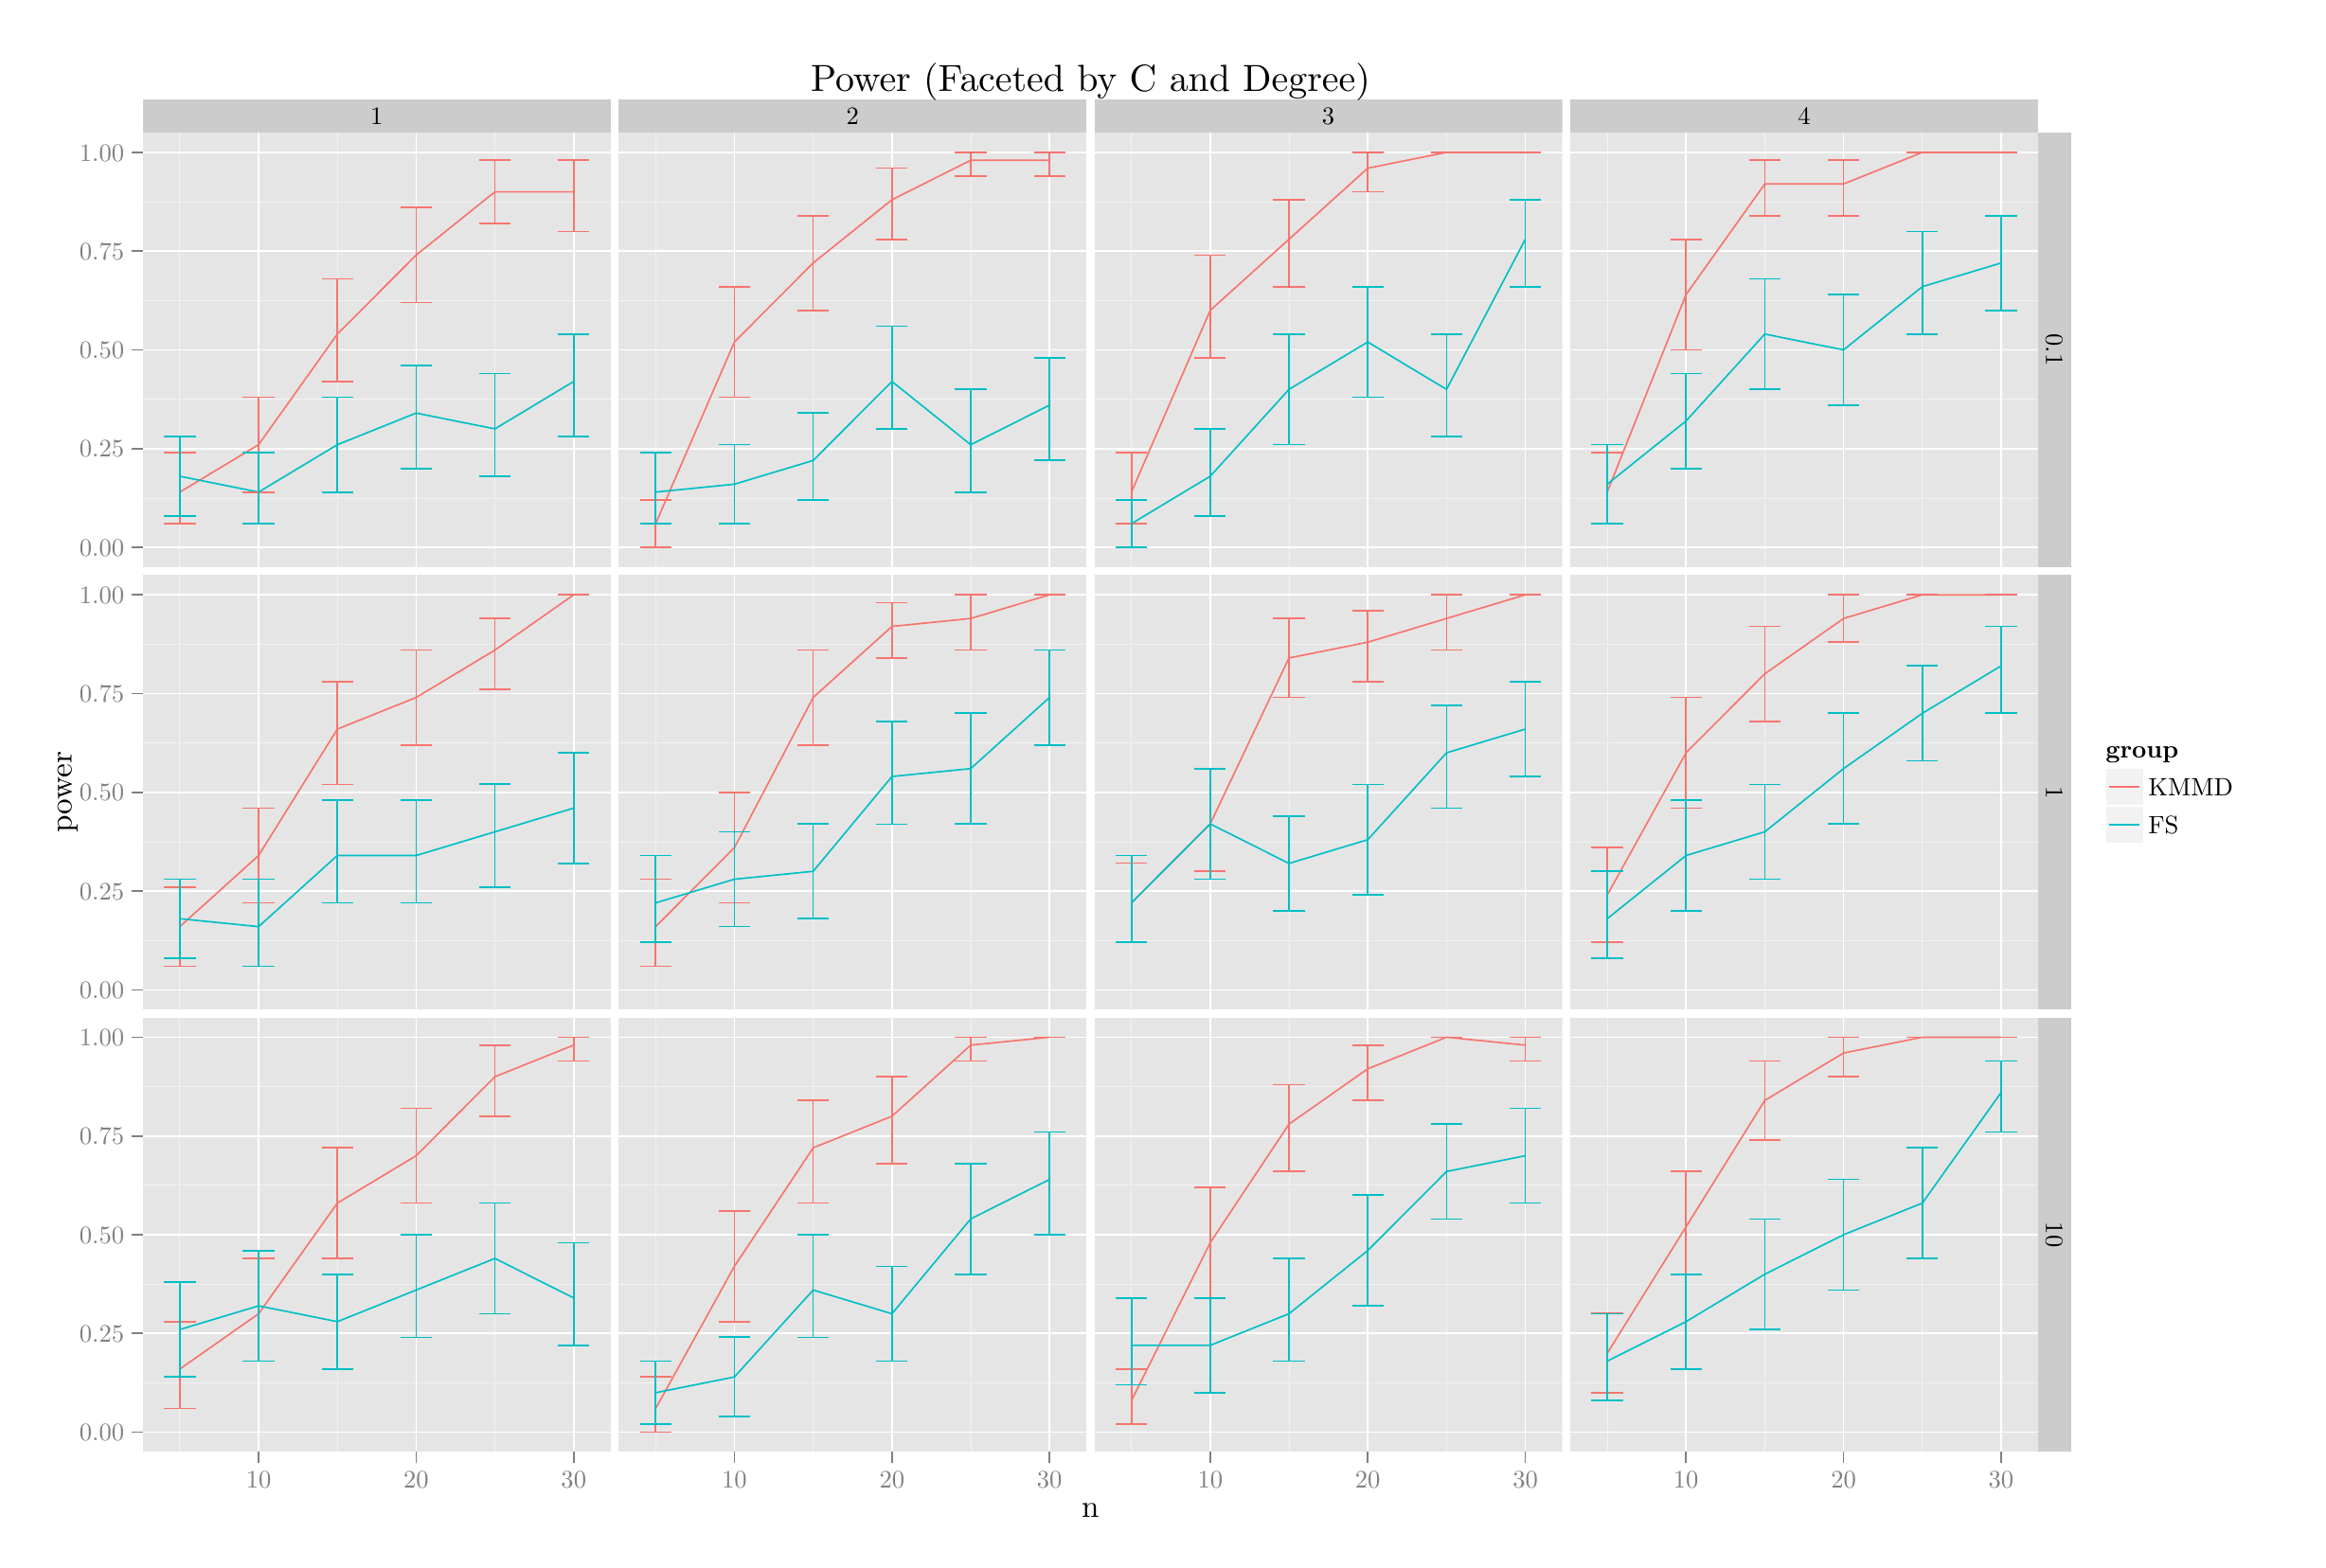
\begin{tikzpicture}[x=1pt,y=1pt]
\definecolor[named]{fillColor}{rgb}{1.00,1.00,1.00}
\path[use as bounding box,fill=fillColor,fill opacity=0.00] (0,0) rectangle (867.24,578.16);
\begin{scope}
\path[clip] (  0.00,  0.00) rectangle (867.24,578.16);
\definecolor[named]{drawColor}{rgb}{1.00,1.00,1.00}
\definecolor[named]{fillColor}{rgb}{1.00,1.00,1.00}

\path[draw=drawColor,line width= 0.6pt,line join=round,line cap=round,fill=fillColor] (  0.00, -0.00) rectangle (867.24,578.16);
\end{scope}
\begin{scope}
\path[clip] ( 44.49,537.54) rectangle (223.01,550.17);
\definecolor[named]{fillColor}{rgb}{0.80,0.80,0.80}

\path[fill=fillColor] ( 44.49,537.54) rectangle (223.01,550.17);
\definecolor[named]{drawColor}{rgb}{0.00,0.00,0.00}

\node[text=drawColor,anchor=base,inner sep=0pt, outer sep=0pt, scale=  0.96] at (133.75,540.55) {1};
\end{scope}
\begin{scope}
\path[clip] (226.03,537.54) rectangle (404.56,550.17);
\definecolor[named]{fillColor}{rgb}{0.80,0.80,0.80}

\path[fill=fillColor] (226.03,537.54) rectangle (404.56,550.17);
\definecolor[named]{drawColor}{rgb}{0.00,0.00,0.00}

\node[text=drawColor,anchor=base,inner sep=0pt, outer sep=0pt, scale=  0.96] at (315.29,540.55) {2};
\end{scope}
\begin{scope}
\path[clip] (407.57,537.54) rectangle (586.10,550.17);
\definecolor[named]{fillColor}{rgb}{0.80,0.80,0.80}

\path[fill=fillColor] (407.57,537.54) rectangle (586.10,550.17);
\definecolor[named]{drawColor}{rgb}{0.00,0.00,0.00}

\node[text=drawColor,anchor=base,inner sep=0pt, outer sep=0pt, scale=  0.96] at (496.83,540.55) {3};
\end{scope}
\begin{scope}
\path[clip] (589.11,537.54) rectangle (767.64,550.17);
\definecolor[named]{fillColor}{rgb}{0.80,0.80,0.80}

\path[fill=fillColor] (589.11,537.54) rectangle (767.64,550.17);
\definecolor[named]{drawColor}{rgb}{0.00,0.00,0.00}

\node[text=drawColor,anchor=base,inner sep=0pt, outer sep=0pt, scale=  0.96] at (678.37,540.55) {4};
\end{scope}
\begin{scope}
\path[clip] ( 44.49,371.71) rectangle (223.01,537.54);
\definecolor[named]{fillColor}{rgb}{0.90,0.90,0.90}

\path[fill=fillColor] ( 44.49,371.71) rectangle (223.01,537.54);
\definecolor[named]{drawColor}{rgb}{0.95,0.95,0.95}

\path[draw=drawColor,line width= 0.3pt,line join=round] ( 44.49,398.09) --
	(223.01,398.09);

\path[draw=drawColor,line width= 0.3pt,line join=round] ( 44.49,435.78) --
	(223.01,435.78);

\path[draw=drawColor,line width= 0.3pt,line join=round] ( 44.49,473.47) --
	(223.01,473.47);

\path[draw=drawColor,line width= 0.3pt,line join=round] ( 44.49,511.16) --
	(223.01,511.16);

\path[draw=drawColor,line width= 0.3pt,line join=round] ( 58.61,371.71) --
	( 58.61,537.54);

\path[draw=drawColor,line width= 0.3pt,line join=round] (118.72,371.71) --
	(118.72,537.54);

\path[draw=drawColor,line width= 0.3pt,line join=round] (178.83,371.71) --
	(178.83,537.54);
\definecolor[named]{drawColor}{rgb}{1.00,1.00,1.00}

\path[draw=drawColor,line width= 0.6pt,line join=round] ( 44.49,379.25) --
	(223.01,379.25);

\path[draw=drawColor,line width= 0.6pt,line join=round] ( 44.49,416.94) --
	(223.01,416.94);

\path[draw=drawColor,line width= 0.6pt,line join=round] ( 44.49,454.63) --
	(223.01,454.63);

\path[draw=drawColor,line width= 0.6pt,line join=round] ( 44.49,492.31) --
	(223.01,492.31);

\path[draw=drawColor,line width= 0.6pt,line join=round] ( 44.49,530.00) --
	(223.01,530.00);

\path[draw=drawColor,line width= 0.6pt,line join=round] ( 88.67,371.71) --
	( 88.67,537.54);

\path[draw=drawColor,line width= 0.6pt,line join=round] (148.78,371.71) --
	(148.78,537.54);

\path[draw=drawColor,line width= 0.6pt,line join=round] (208.89,371.71) --
	(208.89,537.54);
\definecolor[named]{drawColor}{rgb}{0.97,0.46,0.43}

\path[draw=drawColor,line width= 0.6pt,line join=round] ( 58.61,400.36) --
	( 88.67,418.45) --
	(118.72,460.66) --
	(148.78,490.81) --
	(178.83,514.93) --
	(208.89,514.93);
\definecolor[named]{drawColor}{rgb}{0.00,0.75,0.77}

\path[draw=drawColor,line width= 0.6pt,line join=round] ( 58.61,406.39) --
	( 88.67,400.36) --
	(118.72,418.45) --
	(148.78,430.51) --
	(178.83,424.48) --
	(208.89,442.57);
\definecolor[named]{drawColor}{rgb}{0.97,0.46,0.43}

\path[draw=drawColor,line width= 0.6pt,line join=round] ( 52.60,415.43) --
	( 64.62,415.43);

\path[draw=drawColor,line width= 0.6pt,line join=round] ( 58.61,415.43) --
	( 58.61,388.30);

\path[draw=drawColor,line width= 0.6pt,line join=round] ( 52.60,388.30) --
	( 64.62,388.30);

\path[draw=drawColor,line width= 0.6pt,line join=round] ( 82.66,436.54) --
	( 94.68,436.54);

\path[draw=drawColor,line width= 0.6pt,line join=round] ( 88.67,436.54) --
	( 88.67,400.36);

\path[draw=drawColor,line width= 0.6pt,line join=round] ( 82.66,400.36) --
	( 94.68,400.36);

\path[draw=drawColor,line width= 0.6pt,line join=round] (112.71,481.76) --
	(124.73,481.76);

\path[draw=drawColor,line width= 0.6pt,line join=round] (118.72,481.76) --
	(118.72,442.57);

\path[draw=drawColor,line width= 0.6pt,line join=round] (112.71,442.57) --
	(124.73,442.57);

\path[draw=drawColor,line width= 0.6pt,line join=round] (142.77,508.90) --
	(154.79,508.90);

\path[draw=drawColor,line width= 0.6pt,line join=round] (148.78,508.90) --
	(148.78,472.72);

\path[draw=drawColor,line width= 0.6pt,line join=round] (142.77,472.72) --
	(154.79,472.72);

\path[draw=drawColor,line width= 0.6pt,line join=round] (172.82,526.99) --
	(184.84,526.99);

\path[draw=drawColor,line width= 0.6pt,line join=round] (178.83,526.99) --
	(178.83,502.87);

\path[draw=drawColor,line width= 0.6pt,line join=round] (172.82,502.87) --
	(184.84,502.87);

\path[draw=drawColor,line width= 0.6pt,line join=round] (202.88,526.99) --
	(214.90,526.99);

\path[draw=drawColor,line width= 0.6pt,line join=round] (208.89,526.99) --
	(208.89,499.85);

\path[draw=drawColor,line width= 0.6pt,line join=round] (202.88,499.85) --
	(214.90,499.85);
\definecolor[named]{drawColor}{rgb}{0.00,0.75,0.77}

\path[draw=drawColor,line width= 0.6pt,line join=round] ( 52.60,421.54) --
	( 64.62,421.54);

\path[draw=drawColor,line width= 0.6pt,line join=round] ( 58.61,421.54) --
	( 58.61,391.31);

\path[draw=drawColor,line width= 0.6pt,line join=round] ( 52.60,391.31) --
	( 64.62,391.31);

\path[draw=drawColor,line width= 0.6pt,line join=round] ( 82.66,415.43) --
	( 94.68,415.43);

\path[draw=drawColor,line width= 0.6pt,line join=round] ( 88.67,415.43) --
	( 88.67,388.30);

\path[draw=drawColor,line width= 0.6pt,line join=round] ( 82.66,388.30) --
	( 94.68,388.30);

\path[draw=drawColor,line width= 0.6pt,line join=round] (112.71,436.54) --
	(124.73,436.54);

\path[draw=drawColor,line width= 0.6pt,line join=round] (118.72,436.54) --
	(118.72,400.36);

\path[draw=drawColor,line width= 0.6pt,line join=round] (112.71,400.36) --
	(124.73,400.36);

\path[draw=drawColor,line width= 0.6pt,line join=round] (142.77,448.67) --
	(154.79,448.67);

\path[draw=drawColor,line width= 0.6pt,line join=round] (148.78,448.67) --
	(148.78,409.40);

\path[draw=drawColor,line width= 0.6pt,line join=round] (142.77,409.40) --
	(154.79,409.40);

\path[draw=drawColor,line width= 0.6pt,line join=round] (172.82,445.58) --
	(184.84,445.58);

\path[draw=drawColor,line width= 0.6pt,line join=round] (178.83,445.58) --
	(178.83,406.39);

\path[draw=drawColor,line width= 0.6pt,line join=round] (172.82,406.39) --
	(184.84,406.39);

\path[draw=drawColor,line width= 0.6pt,line join=round] (202.88,460.66) --
	(214.90,460.66);

\path[draw=drawColor,line width= 0.6pt,line join=round] (208.89,460.66) --
	(208.89,421.46);

\path[draw=drawColor,line width= 0.6pt,line join=round] (202.88,421.46) --
	(214.90,421.46);
\end{scope}
\begin{scope}
\path[clip] ( 44.49,202.87) rectangle (223.01,368.70);
\definecolor[named]{fillColor}{rgb}{0.90,0.90,0.90}

\path[fill=fillColor] ( 44.49,202.87) rectangle (223.01,368.70);
\definecolor[named]{drawColor}{rgb}{0.95,0.95,0.95}

\path[draw=drawColor,line width= 0.3pt,line join=round] ( 44.49,229.26) --
	(223.01,229.26);

\path[draw=drawColor,line width= 0.3pt,line join=round] ( 44.49,266.94) --
	(223.01,266.94);

\path[draw=drawColor,line width= 0.3pt,line join=round] ( 44.49,304.63) --
	(223.01,304.63);

\path[draw=drawColor,line width= 0.3pt,line join=round] ( 44.49,342.32) --
	(223.01,342.32);

\path[draw=drawColor,line width= 0.3pt,line join=round] ( 58.61,202.87) --
	( 58.61,368.70);

\path[draw=drawColor,line width= 0.3pt,line join=round] (118.72,202.87) --
	(118.72,368.70);

\path[draw=drawColor,line width= 0.3pt,line join=round] (178.83,202.87) --
	(178.83,368.70);
\definecolor[named]{drawColor}{rgb}{1.00,1.00,1.00}

\path[draw=drawColor,line width= 0.6pt,line join=round] ( 44.49,210.41) --
	(223.01,210.41);

\path[draw=drawColor,line width= 0.6pt,line join=round] ( 44.49,248.10) --
	(223.01,248.10);

\path[draw=drawColor,line width= 0.6pt,line join=round] ( 44.49,285.79) --
	(223.01,285.79);

\path[draw=drawColor,line width= 0.6pt,line join=round] ( 44.49,323.48) --
	(223.01,323.48);

\path[draw=drawColor,line width= 0.6pt,line join=round] ( 44.49,361.16) --
	(223.01,361.16);

\path[draw=drawColor,line width= 0.6pt,line join=round] ( 88.67,202.87) --
	( 88.67,368.70);

\path[draw=drawColor,line width= 0.6pt,line join=round] (148.78,202.87) --
	(148.78,368.70);

\path[draw=drawColor,line width= 0.6pt,line join=round] (208.89,202.87) --
	(208.89,368.70);
\definecolor[named]{drawColor}{rgb}{0.97,0.46,0.43}

\path[draw=drawColor,line width= 0.6pt,line join=round] ( 58.61,234.53) --
	( 88.67,261.67) --
	(118.72,309.91) --
	(148.78,321.97) --
	(178.83,340.06) --
	(208.89,361.16);
\definecolor[named]{drawColor}{rgb}{0.00,0.75,0.77}

\path[draw=drawColor,line width= 0.6pt,line join=round] ( 58.61,237.55) --
	( 88.67,234.53) --
	(118.72,261.67) --
	(148.78,261.67) --
	(178.83,270.71) --
	(208.89,279.76);
\definecolor[named]{drawColor}{rgb}{0.97,0.46,0.43}

\path[draw=drawColor,line width= 0.6pt,line join=round] ( 52.60,249.61) --
	( 64.62,249.61);

\path[draw=drawColor,line width= 0.6pt,line join=round] ( 58.61,249.61) --
	( 58.61,219.46);

\path[draw=drawColor,line width= 0.6pt,line join=round] ( 52.60,219.46) --
	( 64.62,219.46);

\path[draw=drawColor,line width= 0.6pt,line join=round] ( 82.66,279.76) --
	( 94.68,279.76);

\path[draw=drawColor,line width= 0.6pt,line join=round] ( 88.67,279.76) --
	( 88.67,243.58);

\path[draw=drawColor,line width= 0.6pt,line join=round] ( 82.66,243.58) --
	( 94.68,243.58);

\path[draw=drawColor,line width= 0.6pt,line join=round] (112.71,328.00) --
	(124.73,328.00);

\path[draw=drawColor,line width= 0.6pt,line join=round] (118.72,328.00) --
	(118.72,288.80);

\path[draw=drawColor,line width= 0.6pt,line join=round] (112.71,288.80) --
	(124.73,288.80);

\path[draw=drawColor,line width= 0.6pt,line join=round] (142.77,340.06) --
	(154.79,340.06);

\path[draw=drawColor,line width= 0.6pt,line join=round] (148.78,340.06) --
	(148.78,303.88);

\path[draw=drawColor,line width= 0.6pt,line join=round] (142.77,303.88) --
	(154.79,303.88);

\path[draw=drawColor,line width= 0.6pt,line join=round] (172.82,352.12) --
	(184.84,352.12);

\path[draw=drawColor,line width= 0.6pt,line join=round] (178.83,352.12) --
	(178.83,324.98);

\path[draw=drawColor,line width= 0.6pt,line join=round] (172.82,324.98) --
	(184.84,324.98);

\path[draw=drawColor,line width= 0.6pt,line join=round] (202.88,361.16) --
	(214.90,361.16);

\path[draw=drawColor,line width= 0.6pt,line join=round] (208.89,361.16) --
	(208.89,361.16);

\path[draw=drawColor,line width= 0.6pt,line join=round] (202.88,361.16) --
	(214.90,361.16);
\definecolor[named]{drawColor}{rgb}{0.00,0.75,0.77}

\path[draw=drawColor,line width= 0.6pt,line join=round] ( 52.60,252.70) --
	( 64.62,252.70);

\path[draw=drawColor,line width= 0.6pt,line join=round] ( 58.61,252.70) --
	( 58.61,222.47);

\path[draw=drawColor,line width= 0.6pt,line join=round] ( 52.60,222.47) --
	( 64.62,222.47);

\path[draw=drawColor,line width= 0.6pt,line join=round] ( 82.66,252.62) --
	( 94.68,252.62);

\path[draw=drawColor,line width= 0.6pt,line join=round] ( 88.67,252.62) --
	( 88.67,219.46);

\path[draw=drawColor,line width= 0.6pt,line join=round] ( 82.66,219.46) --
	( 94.68,219.46);

\path[draw=drawColor,line width= 0.6pt,line join=round] (112.71,282.77) --
	(124.73,282.77);

\path[draw=drawColor,line width= 0.6pt,line join=round] (118.72,282.77) --
	(118.72,243.58);

\path[draw=drawColor,line width= 0.6pt,line join=round] (112.71,243.58) --
	(124.73,243.58);

\path[draw=drawColor,line width= 0.6pt,line join=round] (142.77,282.77) --
	(154.79,282.77);

\path[draw=drawColor,line width= 0.6pt,line join=round] (148.78,282.77) --
	(148.78,243.58);

\path[draw=drawColor,line width= 0.6pt,line join=round] (142.77,243.58) --
	(154.79,243.58);

\path[draw=drawColor,line width= 0.6pt,line join=round] (172.82,288.88) --
	(184.84,288.88);

\path[draw=drawColor,line width= 0.6pt,line join=round] (178.83,288.88) --
	(178.83,249.61);

\path[draw=drawColor,line width= 0.6pt,line join=round] (172.82,249.61) --
	(184.84,249.61);

\path[draw=drawColor,line width= 0.6pt,line join=round] (202.88,300.86) --
	(214.90,300.86);

\path[draw=drawColor,line width= 0.6pt,line join=round] (208.89,300.86) --
	(208.89,258.65);

\path[draw=drawColor,line width= 0.6pt,line join=round] (202.88,258.65) --
	(214.90,258.65);
\end{scope}
\begin{scope}
\path[clip] ( 44.49, 34.03) rectangle (223.01,199.86);
\definecolor[named]{fillColor}{rgb}{0.90,0.90,0.90}

\path[fill=fillColor] ( 44.49, 34.03) rectangle (223.01,199.86);
\definecolor[named]{drawColor}{rgb}{0.95,0.95,0.95}

\path[draw=drawColor,line width= 0.3pt,line join=round] ( 44.49, 60.42) --
	(223.01, 60.42);

\path[draw=drawColor,line width= 0.3pt,line join=round] ( 44.49, 98.10) --
	(223.01, 98.10);

\path[draw=drawColor,line width= 0.3pt,line join=round] ( 44.49,135.79) --
	(223.01,135.79);

\path[draw=drawColor,line width= 0.3pt,line join=round] ( 44.49,173.48) --
	(223.01,173.48);

\path[draw=drawColor,line width= 0.3pt,line join=round] ( 58.61, 34.03) --
	( 58.61,199.86);

\path[draw=drawColor,line width= 0.3pt,line join=round] (118.72, 34.03) --
	(118.72,199.86);

\path[draw=drawColor,line width= 0.3pt,line join=round] (178.83, 34.03) --
	(178.83,199.86);
\definecolor[named]{drawColor}{rgb}{1.00,1.00,1.00}

\path[draw=drawColor,line width= 0.6pt,line join=round] ( 44.49, 41.57) --
	(223.01, 41.57);

\path[draw=drawColor,line width= 0.6pt,line join=round] ( 44.49, 79.26) --
	(223.01, 79.26);

\path[draw=drawColor,line width= 0.6pt,line join=round] ( 44.49,116.95) --
	(223.01,116.95);

\path[draw=drawColor,line width= 0.6pt,line join=round] ( 44.49,154.64) --
	(223.01,154.64);

\path[draw=drawColor,line width= 0.6pt,line join=round] ( 44.49,192.32) --
	(223.01,192.32);

\path[draw=drawColor,line width= 0.6pt,line join=round] ( 88.67, 34.03) --
	( 88.67,199.86);

\path[draw=drawColor,line width= 0.6pt,line join=round] (148.78, 34.03) --
	(148.78,199.86);

\path[draw=drawColor,line width= 0.6pt,line join=round] (208.89, 34.03) --
	(208.89,199.86);
\definecolor[named]{drawColor}{rgb}{0.97,0.46,0.43}

\path[draw=drawColor,line width= 0.6pt,line join=round] ( 58.61, 65.69) --
	( 88.67, 86.80) --
	(118.72,129.01) --
	(148.78,147.10) --
	(178.83,177.25) --
	(208.89,189.31);
\definecolor[named]{drawColor}{rgb}{0.00,0.75,0.77}

\path[draw=drawColor,line width= 0.6pt,line join=round] ( 58.61, 80.77) --
	( 88.67, 89.81) --
	(118.72, 83.78) --
	(148.78, 95.84) --
	(178.83,107.90) --
	(208.89, 92.83);
\definecolor[named]{drawColor}{rgb}{0.97,0.46,0.43}

\path[draw=drawColor,line width= 0.6pt,line join=round] ( 52.60, 83.78) --
	( 64.62, 83.78);

\path[draw=drawColor,line width= 0.6pt,line join=round] ( 58.61, 83.78) --
	( 58.61, 50.62);

\path[draw=drawColor,line width= 0.6pt,line join=round] ( 52.60, 50.62) --
	( 64.62, 50.62);

\path[draw=drawColor,line width= 0.6pt,line join=round] ( 82.66,107.90) --
	( 94.68,107.90);

\path[draw=drawColor,line width= 0.6pt,line join=round] ( 88.67,107.90) --
	( 88.67, 68.71);

\path[draw=drawColor,line width= 0.6pt,line join=round] ( 82.66, 68.71) --
	( 94.68, 68.71);

\path[draw=drawColor,line width= 0.6pt,line join=round] (112.71,150.11) --
	(124.73,150.11);

\path[draw=drawColor,line width= 0.6pt,line join=round] (118.72,150.11) --
	(118.72,107.90);

\path[draw=drawColor,line width= 0.6pt,line join=round] (112.71,107.90) --
	(124.73,107.90);

\path[draw=drawColor,line width= 0.6pt,line join=round] (142.77,165.19) --
	(154.79,165.19);

\path[draw=drawColor,line width= 0.6pt,line join=round] (148.78,165.19) --
	(148.78,129.01);

\path[draw=drawColor,line width= 0.6pt,line join=round] (142.77,129.01) --
	(154.79,129.01);

\path[draw=drawColor,line width= 0.6pt,line join=round] (172.82,189.31) --
	(184.84,189.31);

\path[draw=drawColor,line width= 0.6pt,line join=round] (178.83,189.31) --
	(178.83,162.17);

\path[draw=drawColor,line width= 0.6pt,line join=round] (172.82,162.17) --
	(184.84,162.17);

\path[draw=drawColor,line width= 0.6pt,line join=round] (202.88,192.32) --
	(214.90,192.32);

\path[draw=drawColor,line width= 0.6pt,line join=round] (208.89,192.32) --
	(208.89,183.28);

\path[draw=drawColor,line width= 0.6pt,line join=round] (202.88,183.28) --
	(214.90,183.28);
\definecolor[named]{drawColor}{rgb}{0.00,0.75,0.77}

\path[draw=drawColor,line width= 0.6pt,line join=round] ( 52.60, 98.86) --
	( 64.62, 98.86);

\path[draw=drawColor,line width= 0.6pt,line join=round] ( 58.61, 98.86) --
	( 58.61, 62.68);

\path[draw=drawColor,line width= 0.6pt,line join=round] ( 52.60, 62.68) --
	( 64.62, 62.68);

\path[draw=drawColor,line width= 0.6pt,line join=round] ( 82.66,110.92) --
	( 94.68,110.92);

\path[draw=drawColor,line width= 0.6pt,line join=round] ( 88.67,110.92) --
	( 88.67, 68.71);

\path[draw=drawColor,line width= 0.6pt,line join=round] ( 82.66, 68.71) --
	( 94.68, 68.71);

\path[draw=drawColor,line width= 0.6pt,line join=round] (112.71,101.87) --
	(124.73,101.87);

\path[draw=drawColor,line width= 0.6pt,line join=round] (118.72,101.87) --
	(118.72, 65.62);

\path[draw=drawColor,line width= 0.6pt,line join=round] (112.71, 65.62) --
	(124.73, 65.62);

\path[draw=drawColor,line width= 0.6pt,line join=round] (142.77,116.95) --
	(154.79,116.95);

\path[draw=drawColor,line width= 0.6pt,line join=round] (148.78,116.95) --
	(148.78, 77.75);

\path[draw=drawColor,line width= 0.6pt,line join=round] (142.77, 77.75) --
	(154.79, 77.75);

\path[draw=drawColor,line width= 0.6pt,line join=round] (172.82,129.01) --
	(184.84,129.01);

\path[draw=drawColor,line width= 0.6pt,line join=round] (178.83,129.01) --
	(178.83, 86.80);

\path[draw=drawColor,line width= 0.6pt,line join=round] (172.82, 86.80) --
	(184.84, 86.80);

\path[draw=drawColor,line width= 0.6pt,line join=round] (202.88,113.93) --
	(214.90,113.93);

\path[draw=drawColor,line width= 0.6pt,line join=round] (208.89,113.93) --
	(208.89, 74.74);

\path[draw=drawColor,line width= 0.6pt,line join=round] (202.88, 74.74) --
	(214.90, 74.74);
\end{scope}
\begin{scope}
\path[clip] (226.03,371.71) rectangle (404.56,537.54);
\definecolor[named]{fillColor}{rgb}{0.90,0.90,0.90}

\path[fill=fillColor] (226.03,371.71) rectangle (404.56,537.54);
\definecolor[named]{drawColor}{rgb}{0.95,0.95,0.95}

\path[draw=drawColor,line width= 0.3pt,line join=round] (226.03,398.09) --
	(404.56,398.09);

\path[draw=drawColor,line width= 0.3pt,line join=round] (226.03,435.78) --
	(404.56,435.78);

\path[draw=drawColor,line width= 0.3pt,line join=round] (226.03,473.47) --
	(404.56,473.47);

\path[draw=drawColor,line width= 0.3pt,line join=round] (226.03,511.16) --
	(404.56,511.16);

\path[draw=drawColor,line width= 0.3pt,line join=round] (240.15,371.71) --
	(240.15,537.54);

\path[draw=drawColor,line width= 0.3pt,line join=round] (300.26,371.71) --
	(300.26,537.54);

\path[draw=drawColor,line width= 0.3pt,line join=round] (360.37,371.71) --
	(360.37,537.54);
\definecolor[named]{drawColor}{rgb}{1.00,1.00,1.00}

\path[draw=drawColor,line width= 0.6pt,line join=round] (226.03,379.25) --
	(404.56,379.25);

\path[draw=drawColor,line width= 0.6pt,line join=round] (226.03,416.94) --
	(404.56,416.94);

\path[draw=drawColor,line width= 0.6pt,line join=round] (226.03,454.63) --
	(404.56,454.63);

\path[draw=drawColor,line width= 0.6pt,line join=round] (226.03,492.31) --
	(404.56,492.31);

\path[draw=drawColor,line width= 0.6pt,line join=round] (226.03,530.00) --
	(404.56,530.00);

\path[draw=drawColor,line width= 0.6pt,line join=round] (270.21,371.71) --
	(270.21,537.54);

\path[draw=drawColor,line width= 0.6pt,line join=round] (330.32,371.71) --
	(330.32,537.54);

\path[draw=drawColor,line width= 0.6pt,line join=round] (390.43,371.71) --
	(390.43,537.54);
\definecolor[named]{drawColor}{rgb}{0.97,0.46,0.43}

\path[draw=drawColor,line width= 0.6pt,line join=round] (240.15,388.30) --
	(270.21,457.64) --
	(300.26,487.79) --
	(330.32,511.91) --
	(360.37,526.99) --
	(390.43,526.99);
\definecolor[named]{drawColor}{rgb}{0.00,0.75,0.77}

\path[draw=drawColor,line width= 0.6pt,line join=round] (240.15,400.36) --
	(270.21,403.37) --
	(300.26,412.42) --
	(330.32,442.57) --
	(360.37,418.45) --
	(390.43,433.52);
\definecolor[named]{drawColor}{rgb}{0.97,0.46,0.43}

\path[draw=drawColor,line width= 0.6pt,line join=round] (234.14,397.34) --
	(246.16,397.34);

\path[draw=drawColor,line width= 0.6pt,line join=round] (240.15,397.34) --
	(240.15,379.25);

\path[draw=drawColor,line width= 0.6pt,line join=round] (234.14,379.25) --
	(246.16,379.25);

\path[draw=drawColor,line width= 0.6pt,line join=round] (264.20,478.75) --
	(276.22,478.75);

\path[draw=drawColor,line width= 0.6pt,line join=round] (270.21,478.75) --
	(270.21,436.54);

\path[draw=drawColor,line width= 0.6pt,line join=round] (264.20,436.54) --
	(276.22,436.54);

\path[draw=drawColor,line width= 0.6pt,line join=round] (294.25,505.88) --
	(306.27,505.88);

\path[draw=drawColor,line width= 0.6pt,line join=round] (300.26,505.88) --
	(300.26,469.70);

\path[draw=drawColor,line width= 0.6pt,line join=round] (294.25,469.70) --
	(306.27,469.70);

\path[draw=drawColor,line width= 0.6pt,line join=round] (324.31,523.97) --
	(336.33,523.97);

\path[draw=drawColor,line width= 0.6pt,line join=round] (330.32,523.97) --
	(330.32,496.84);

\path[draw=drawColor,line width= 0.6pt,line join=round] (324.31,496.84) --
	(336.33,496.84);

\path[draw=drawColor,line width= 0.6pt,line join=round] (354.36,530.00) --
	(366.38,530.00);

\path[draw=drawColor,line width= 0.6pt,line join=round] (360.37,530.00) --
	(360.37,520.96);

\path[draw=drawColor,line width= 0.6pt,line join=round] (354.36,520.96) --
	(366.38,520.96);

\path[draw=drawColor,line width= 0.6pt,line join=round] (384.42,530.00) --
	(396.44,530.00);

\path[draw=drawColor,line width= 0.6pt,line join=round] (390.43,530.00) --
	(390.43,520.96);

\path[draw=drawColor,line width= 0.6pt,line join=round] (384.42,520.96) --
	(396.44,520.96);
\definecolor[named]{drawColor}{rgb}{0.00,0.75,0.77}

\path[draw=drawColor,line width= 0.6pt,line join=round] (234.14,415.43) --
	(246.16,415.43);

\path[draw=drawColor,line width= 0.6pt,line join=round] (240.15,415.43) --
	(240.15,388.30);

\path[draw=drawColor,line width= 0.6pt,line join=round] (234.14,388.30) --
	(246.16,388.30);

\path[draw=drawColor,line width= 0.6pt,line join=round] (264.20,418.45) --
	(276.22,418.45);

\path[draw=drawColor,line width= 0.6pt,line join=round] (270.21,418.45) --
	(270.21,388.30);

\path[draw=drawColor,line width= 0.6pt,line join=round] (264.20,388.30) --
	(276.22,388.30);

\path[draw=drawColor,line width= 0.6pt,line join=round] (294.25,430.51) --
	(306.27,430.51);

\path[draw=drawColor,line width= 0.6pt,line join=round] (300.26,430.51) --
	(300.26,397.34);

\path[draw=drawColor,line width= 0.6pt,line join=round] (294.25,397.34) --
	(306.27,397.34);

\path[draw=drawColor,line width= 0.6pt,line join=round] (324.31,463.67) --
	(336.33,463.67);

\path[draw=drawColor,line width= 0.6pt,line join=round] (330.32,463.67) --
	(330.32,424.48);

\path[draw=drawColor,line width= 0.6pt,line join=round] (324.31,424.48) --
	(336.33,424.48);

\path[draw=drawColor,line width= 0.6pt,line join=round] (354.36,439.55) --
	(366.38,439.55);

\path[draw=drawColor,line width= 0.6pt,line join=round] (360.37,439.55) --
	(360.37,400.36);

\path[draw=drawColor,line width= 0.6pt,line join=round] (354.36,400.36) --
	(366.38,400.36);

\path[draw=drawColor,line width= 0.6pt,line join=round] (384.42,451.61) --
	(396.44,451.61);

\path[draw=drawColor,line width= 0.6pt,line join=round] (390.43,451.61) --
	(390.43,412.42);

\path[draw=drawColor,line width= 0.6pt,line join=round] (384.42,412.42) --
	(396.44,412.42);
\end{scope}
\begin{scope}
\path[clip] (226.03,202.87) rectangle (404.56,368.70);
\definecolor[named]{fillColor}{rgb}{0.90,0.90,0.90}

\path[fill=fillColor] (226.03,202.87) rectangle (404.56,368.70);
\definecolor[named]{drawColor}{rgb}{0.95,0.95,0.95}

\path[draw=drawColor,line width= 0.3pt,line join=round] (226.03,229.26) --
	(404.56,229.26);

\path[draw=drawColor,line width= 0.3pt,line join=round] (226.03,266.94) --
	(404.56,266.94);

\path[draw=drawColor,line width= 0.3pt,line join=round] (226.03,304.63) --
	(404.56,304.63);

\path[draw=drawColor,line width= 0.3pt,line join=round] (226.03,342.32) --
	(404.56,342.32);

\path[draw=drawColor,line width= 0.3pt,line join=round] (240.15,202.87) --
	(240.15,368.70);

\path[draw=drawColor,line width= 0.3pt,line join=round] (300.26,202.87) --
	(300.26,368.70);

\path[draw=drawColor,line width= 0.3pt,line join=round] (360.37,202.87) --
	(360.37,368.70);
\definecolor[named]{drawColor}{rgb}{1.00,1.00,1.00}

\path[draw=drawColor,line width= 0.6pt,line join=round] (226.03,210.41) --
	(404.56,210.41);

\path[draw=drawColor,line width= 0.6pt,line join=round] (226.03,248.10) --
	(404.56,248.10);

\path[draw=drawColor,line width= 0.6pt,line join=round] (226.03,285.79) --
	(404.56,285.79);

\path[draw=drawColor,line width= 0.6pt,line join=round] (226.03,323.48) --
	(404.56,323.48);

\path[draw=drawColor,line width= 0.6pt,line join=round] (226.03,361.16) --
	(404.56,361.16);

\path[draw=drawColor,line width= 0.6pt,line join=round] (270.21,202.87) --
	(270.21,368.70);

\path[draw=drawColor,line width= 0.6pt,line join=round] (330.32,202.87) --
	(330.32,368.70);

\path[draw=drawColor,line width= 0.6pt,line join=round] (390.43,202.87) --
	(390.43,368.70);
\definecolor[named]{drawColor}{rgb}{0.97,0.46,0.43}

\path[draw=drawColor,line width= 0.6pt,line join=round] (240.15,234.53) --
	(270.21,264.68) --
	(300.26,321.97) --
	(330.32,349.10) --
	(360.37,352.12) --
	(390.43,361.16);
\definecolor[named]{drawColor}{rgb}{0.00,0.75,0.77}

\path[draw=drawColor,line width= 0.6pt,line join=round] (240.15,243.58) --
	(270.21,252.62) --
	(300.26,255.64) --
	(330.32,291.82) --
	(360.37,294.83) --
	(390.43,321.97);
\definecolor[named]{drawColor}{rgb}{0.97,0.46,0.43}

\path[draw=drawColor,line width= 0.6pt,line join=round] (234.14,252.62) --
	(246.16,252.62);

\path[draw=drawColor,line width= 0.6pt,line join=round] (240.15,252.62) --
	(240.15,219.46);

\path[draw=drawColor,line width= 0.6pt,line join=round] (234.14,219.46) --
	(246.16,219.46);

\path[draw=drawColor,line width= 0.6pt,line join=round] (264.20,285.79) --
	(276.22,285.79);

\path[draw=drawColor,line width= 0.6pt,line join=round] (270.21,285.79) --
	(270.21,243.58);

\path[draw=drawColor,line width= 0.6pt,line join=round] (264.20,243.58) --
	(276.22,243.58);

\path[draw=drawColor,line width= 0.6pt,line join=round] (294.25,340.06) --
	(306.27,340.06);

\path[draw=drawColor,line width= 0.6pt,line join=round] (300.26,340.06) --
	(300.26,303.88);

\path[draw=drawColor,line width= 0.6pt,line join=round] (294.25,303.88) --
	(306.27,303.88);

\path[draw=drawColor,line width= 0.6pt,line join=round] (324.31,358.15) --
	(336.33,358.15);

\path[draw=drawColor,line width= 0.6pt,line join=round] (330.32,358.15) --
	(330.32,337.04);

\path[draw=drawColor,line width= 0.6pt,line join=round] (324.31,337.04) --
	(336.33,337.04);

\path[draw=drawColor,line width= 0.6pt,line join=round] (354.36,361.16) --
	(366.38,361.16);

\path[draw=drawColor,line width= 0.6pt,line join=round] (360.37,361.16) --
	(360.37,340.06);

\path[draw=drawColor,line width= 0.6pt,line join=round] (354.36,340.06) --
	(366.38,340.06);

\path[draw=drawColor,line width= 0.6pt,line join=round] (384.42,361.16) --
	(396.44,361.16);

\path[draw=drawColor,line width= 0.6pt,line join=round] (390.43,361.16) --
	(390.43,361.16);

\path[draw=drawColor,line width= 0.6pt,line join=round] (384.42,361.16) --
	(396.44,361.16);
\definecolor[named]{drawColor}{rgb}{0.00,0.75,0.77}

\path[draw=drawColor,line width= 0.6pt,line join=round] (234.14,261.67) --
	(246.16,261.67);

\path[draw=drawColor,line width= 0.6pt,line join=round] (240.15,261.67) --
	(240.15,228.50);

\path[draw=drawColor,line width= 0.6pt,line join=round] (234.14,228.50) --
	(246.16,228.50);

\path[draw=drawColor,line width= 0.6pt,line join=round] (264.20,270.71) --
	(276.22,270.71);

\path[draw=drawColor,line width= 0.6pt,line join=round] (270.21,270.71) --
	(270.21,234.53);

\path[draw=drawColor,line width= 0.6pt,line join=round] (264.20,234.53) --
	(276.22,234.53);

\path[draw=drawColor,line width= 0.6pt,line join=round] (294.25,273.73) --
	(306.27,273.73);

\path[draw=drawColor,line width= 0.6pt,line join=round] (300.26,273.73) --
	(300.26,237.55);

\path[draw=drawColor,line width= 0.6pt,line join=round] (294.25,237.55) --
	(306.27,237.55);

\path[draw=drawColor,line width= 0.6pt,line join=round] (324.31,312.92) --
	(336.33,312.92);

\path[draw=drawColor,line width= 0.6pt,line join=round] (330.32,312.92) --
	(330.32,273.65);

\path[draw=drawColor,line width= 0.6pt,line join=round] (324.31,273.65) --
	(336.33,273.65);

\path[draw=drawColor,line width= 0.6pt,line join=round] (354.36,315.94) --
	(366.38,315.94);

\path[draw=drawColor,line width= 0.6pt,line join=round] (360.37,315.94) --
	(360.37,273.73);

\path[draw=drawColor,line width= 0.6pt,line join=round] (354.36,273.73) --
	(366.38,273.73);

\path[draw=drawColor,line width= 0.6pt,line join=round] (384.42,340.06) --
	(396.44,340.06);

\path[draw=drawColor,line width= 0.6pt,line join=round] (390.43,340.06) --
	(390.43,303.80);

\path[draw=drawColor,line width= 0.6pt,line join=round] (384.42,303.80) --
	(396.44,303.80);
\end{scope}
\begin{scope}
\path[clip] (226.03, 34.03) rectangle (404.56,199.86);
\definecolor[named]{fillColor}{rgb}{0.90,0.90,0.90}

\path[fill=fillColor] (226.03, 34.03) rectangle (404.56,199.86);
\definecolor[named]{drawColor}{rgb}{0.95,0.95,0.95}

\path[draw=drawColor,line width= 0.3pt,line join=round] (226.03, 60.42) --
	(404.56, 60.42);

\path[draw=drawColor,line width= 0.3pt,line join=round] (226.03, 98.10) --
	(404.56, 98.10);

\path[draw=drawColor,line width= 0.3pt,line join=round] (226.03,135.79) --
	(404.56,135.79);

\path[draw=drawColor,line width= 0.3pt,line join=round] (226.03,173.48) --
	(404.56,173.48);

\path[draw=drawColor,line width= 0.3pt,line join=round] (240.15, 34.03) --
	(240.15,199.86);

\path[draw=drawColor,line width= 0.3pt,line join=round] (300.26, 34.03) --
	(300.26,199.86);

\path[draw=drawColor,line width= 0.3pt,line join=round] (360.37, 34.03) --
	(360.37,199.86);
\definecolor[named]{drawColor}{rgb}{1.00,1.00,1.00}

\path[draw=drawColor,line width= 0.6pt,line join=round] (226.03, 41.57) --
	(404.56, 41.57);

\path[draw=drawColor,line width= 0.6pt,line join=round] (226.03, 79.26) --
	(404.56, 79.26);

\path[draw=drawColor,line width= 0.6pt,line join=round] (226.03,116.95) --
	(404.56,116.95);

\path[draw=drawColor,line width= 0.6pt,line join=round] (226.03,154.64) --
	(404.56,154.64);

\path[draw=drawColor,line width= 0.6pt,line join=round] (226.03,192.32) --
	(404.56,192.32);

\path[draw=drawColor,line width= 0.6pt,line join=round] (270.21, 34.03) --
	(270.21,199.86);

\path[draw=drawColor,line width= 0.6pt,line join=round] (330.32, 34.03) --
	(330.32,199.86);

\path[draw=drawColor,line width= 0.6pt,line join=round] (390.43, 34.03) --
	(390.43,199.86);
\definecolor[named]{drawColor}{rgb}{0.97,0.46,0.43}

\path[draw=drawColor,line width= 0.6pt,line join=round] (240.15, 50.62) --
	(270.21,104.89) --
	(300.26,150.11) --
	(330.32,162.17) --
	(360.37,189.31) --
	(390.43,192.32);
\definecolor[named]{drawColor}{rgb}{0.00,0.75,0.77}

\path[draw=drawColor,line width= 0.6pt,line join=round] (240.15, 56.65) --
	(270.21, 62.68) --
	(300.26, 95.84) --
	(330.32, 86.80) --
	(360.37,122.98) --
	(390.43,138.05);
\definecolor[named]{drawColor}{rgb}{0.97,0.46,0.43}

\path[draw=drawColor,line width= 0.6pt,line join=round] (234.14, 62.68) --
	(246.16, 62.68);

\path[draw=drawColor,line width= 0.6pt,line join=round] (240.15, 62.68) --
	(240.15, 41.57);

\path[draw=drawColor,line width= 0.6pt,line join=round] (234.14, 41.57) --
	(246.16, 41.57);

\path[draw=drawColor,line width= 0.6pt,line join=round] (264.20,125.99) --
	(276.22,125.99);

\path[draw=drawColor,line width= 0.6pt,line join=round] (270.21,125.99) --
	(270.21, 83.78);

\path[draw=drawColor,line width= 0.6pt,line join=round] (264.20, 83.78) --
	(276.22, 83.78);

\path[draw=drawColor,line width= 0.6pt,line join=round] (294.25,168.20) --
	(306.27,168.20);

\path[draw=drawColor,line width= 0.6pt,line join=round] (300.26,168.20) --
	(300.26,129.01);

\path[draw=drawColor,line width= 0.6pt,line join=round] (294.25,129.01) --
	(306.27,129.01);

\path[draw=drawColor,line width= 0.6pt,line join=round] (324.31,177.25) --
	(336.33,177.25);

\path[draw=drawColor,line width= 0.6pt,line join=round] (330.32,177.25) --
	(330.32,144.08);

\path[draw=drawColor,line width= 0.6pt,line join=round] (324.31,144.08) --
	(336.33,144.08);

\path[draw=drawColor,line width= 0.6pt,line join=round] (354.36,192.32) --
	(366.38,192.32);

\path[draw=drawColor,line width= 0.6pt,line join=round] (360.37,192.32) --
	(360.37,183.28);

\path[draw=drawColor,line width= 0.6pt,line join=round] (354.36,183.28) --
	(366.38,183.28);

\path[draw=drawColor,line width= 0.6pt,line join=round] (384.42,192.32) --
	(396.44,192.32);

\path[draw=drawColor,line width= 0.6pt,line join=round] (390.43,192.32) --
	(390.43,192.32);

\path[draw=drawColor,line width= 0.6pt,line join=round] (384.42,192.32) --
	(396.44,192.32);
\definecolor[named]{drawColor}{rgb}{0.00,0.75,0.77}

\path[draw=drawColor,line width= 0.6pt,line join=round] (234.14, 68.71) --
	(246.16, 68.71);

\path[draw=drawColor,line width= 0.6pt,line join=round] (240.15, 68.71) --
	(240.15, 44.59);

\path[draw=drawColor,line width= 0.6pt,line join=round] (234.14, 44.59) --
	(246.16, 44.59);

\path[draw=drawColor,line width= 0.6pt,line join=round] (264.20, 77.83) --
	(276.22, 77.83);

\path[draw=drawColor,line width= 0.6pt,line join=round] (270.21, 77.83) --
	(270.21, 47.60);

\path[draw=drawColor,line width= 0.6pt,line join=round] (264.20, 47.60) --
	(276.22, 47.60);

\path[draw=drawColor,line width= 0.6pt,line join=round] (294.25,116.95) --
	(306.27,116.95);

\path[draw=drawColor,line width= 0.6pt,line join=round] (300.26,116.95) --
	(300.26, 77.75);

\path[draw=drawColor,line width= 0.6pt,line join=round] (294.25, 77.75) --
	(306.27, 77.75);

\path[draw=drawColor,line width= 0.6pt,line join=round] (324.31,104.89) --
	(336.33,104.89);

\path[draw=drawColor,line width= 0.6pt,line join=round] (330.32,104.89) --
	(330.32, 68.71);

\path[draw=drawColor,line width= 0.6pt,line join=round] (324.31, 68.71) --
	(336.33, 68.71);

\path[draw=drawColor,line width= 0.6pt,line join=round] (354.36,144.16) --
	(366.38,144.16);

\path[draw=drawColor,line width= 0.6pt,line join=round] (360.37,144.16) --
	(360.37,101.87);

\path[draw=drawColor,line width= 0.6pt,line join=round] (354.36,101.87) --
	(366.38,101.87);

\path[draw=drawColor,line width= 0.6pt,line join=round] (384.42,156.14) --
	(396.44,156.14);

\path[draw=drawColor,line width= 0.6pt,line join=round] (390.43,156.14) --
	(390.43,116.95);

\path[draw=drawColor,line width= 0.6pt,line join=round] (384.42,116.95) --
	(396.44,116.95);
\end{scope}
\begin{scope}
\path[clip] (407.57,371.71) rectangle (586.10,537.54);
\definecolor[named]{fillColor}{rgb}{0.90,0.90,0.90}

\path[fill=fillColor] (407.57,371.71) rectangle (586.10,537.54);
\definecolor[named]{drawColor}{rgb}{0.95,0.95,0.95}

\path[draw=drawColor,line width= 0.3pt,line join=round] (407.57,398.09) --
	(586.10,398.09);

\path[draw=drawColor,line width= 0.3pt,line join=round] (407.57,435.78) --
	(586.10,435.78);

\path[draw=drawColor,line width= 0.3pt,line join=round] (407.57,473.47) --
	(586.10,473.47);

\path[draw=drawColor,line width= 0.3pt,line join=round] (407.57,511.16) --
	(586.10,511.16);

\path[draw=drawColor,line width= 0.3pt,line join=round] (421.69,371.71) --
	(421.69,537.54);

\path[draw=drawColor,line width= 0.3pt,line join=round] (481.80,371.71) --
	(481.80,537.54);

\path[draw=drawColor,line width= 0.3pt,line join=round] (541.91,371.71) --
	(541.91,537.54);
\definecolor[named]{drawColor}{rgb}{1.00,1.00,1.00}

\path[draw=drawColor,line width= 0.6pt,line join=round] (407.57,379.25) --
	(586.10,379.25);

\path[draw=drawColor,line width= 0.6pt,line join=round] (407.57,416.94) --
	(586.10,416.94);

\path[draw=drawColor,line width= 0.6pt,line join=round] (407.57,454.63) --
	(586.10,454.63);

\path[draw=drawColor,line width= 0.6pt,line join=round] (407.57,492.31) --
	(586.10,492.31);

\path[draw=drawColor,line width= 0.6pt,line join=round] (407.57,530.00) --
	(586.10,530.00);

\path[draw=drawColor,line width= 0.6pt,line join=round] (451.75,371.71) --
	(451.75,537.54);

\path[draw=drawColor,line width= 0.6pt,line join=round] (511.86,371.71) --
	(511.86,537.54);

\path[draw=drawColor,line width= 0.6pt,line join=round] (571.97,371.71) --
	(571.97,537.54);
\definecolor[named]{drawColor}{rgb}{0.97,0.46,0.43}

\path[draw=drawColor,line width= 0.6pt,line join=round] (421.69,400.36) --
	(451.75,469.70) --
	(481.80,496.84) --
	(511.86,523.97) --
	(541.91,530.00) --
	(571.97,530.00);
\definecolor[named]{drawColor}{rgb}{0.00,0.75,0.77}

\path[draw=drawColor,line width= 0.6pt,line join=round] (421.69,388.30) --
	(451.75,406.39) --
	(481.80,439.55) --
	(511.86,457.64) --
	(541.91,439.55) --
	(571.97,496.84);
\definecolor[named]{drawColor}{rgb}{0.97,0.46,0.43}

\path[draw=drawColor,line width= 0.6pt,line join=round] (415.68,415.43) --
	(427.70,415.43);

\path[draw=drawColor,line width= 0.6pt,line join=round] (421.69,415.43) --
	(421.69,388.30);

\path[draw=drawColor,line width= 0.6pt,line join=round] (415.68,388.30) --
	(427.70,388.30);

\path[draw=drawColor,line width= 0.6pt,line join=round] (445.74,490.81) --
	(457.76,490.81);

\path[draw=drawColor,line width= 0.6pt,line join=round] (451.75,490.81) --
	(451.75,451.61);

\path[draw=drawColor,line width= 0.6pt,line join=round] (445.74,451.61) --
	(457.76,451.61);

\path[draw=drawColor,line width= 0.6pt,line join=round] (475.79,511.91) --
	(487.81,511.91);

\path[draw=drawColor,line width= 0.6pt,line join=round] (481.80,511.91) --
	(481.80,478.75);

\path[draw=drawColor,line width= 0.6pt,line join=round] (475.79,478.75) --
	(487.81,478.75);

\path[draw=drawColor,line width= 0.6pt,line join=round] (505.85,530.00) --
	(517.87,530.00);

\path[draw=drawColor,line width= 0.6pt,line join=round] (511.86,530.00) --
	(511.86,514.93);

\path[draw=drawColor,line width= 0.6pt,line join=round] (505.85,514.93) --
	(517.87,514.93);

\path[draw=drawColor,line width= 0.6pt,line join=round] (535.90,530.00) --
	(547.93,530.00);

\path[draw=drawColor,line width= 0.6pt,line join=round] (541.91,530.00) --
	(541.91,530.00);

\path[draw=drawColor,line width= 0.6pt,line join=round] (535.90,530.00) --
	(547.93,530.00);

\path[draw=drawColor,line width= 0.6pt,line join=round] (565.96,530.00) --
	(577.98,530.00);

\path[draw=drawColor,line width= 0.6pt,line join=round] (571.97,530.00) --
	(571.97,530.00);

\path[draw=drawColor,line width= 0.6pt,line join=round] (565.96,530.00) --
	(577.98,530.00);
\definecolor[named]{drawColor}{rgb}{0.00,0.75,0.77}

\path[draw=drawColor,line width= 0.6pt,line join=round] (415.68,397.34) --
	(427.70,397.34);

\path[draw=drawColor,line width= 0.6pt,line join=round] (421.69,397.34) --
	(421.69,379.25);

\path[draw=drawColor,line width= 0.6pt,line join=round] (415.68,379.25) --
	(427.70,379.25);

\path[draw=drawColor,line width= 0.6pt,line join=round] (445.74,424.48) --
	(457.76,424.48);

\path[draw=drawColor,line width= 0.6pt,line join=round] (451.75,424.48) --
	(451.75,391.31);

\path[draw=drawColor,line width= 0.6pt,line join=round] (445.74,391.31) --
	(457.76,391.31);

\path[draw=drawColor,line width= 0.6pt,line join=round] (475.79,460.66) --
	(487.81,460.66);

\path[draw=drawColor,line width= 0.6pt,line join=round] (481.80,460.66) --
	(481.80,418.45);

\path[draw=drawColor,line width= 0.6pt,line join=round] (475.79,418.45) --
	(487.81,418.45);

\path[draw=drawColor,line width= 0.6pt,line join=round] (505.85,478.75) --
	(517.87,478.75);

\path[draw=drawColor,line width= 0.6pt,line join=round] (511.86,478.75) --
	(511.86,436.54);

\path[draw=drawColor,line width= 0.6pt,line join=round] (505.85,436.54) --
	(517.87,436.54);

\path[draw=drawColor,line width= 0.6pt,line join=round] (535.90,460.66) --
	(547.93,460.66);

\path[draw=drawColor,line width= 0.6pt,line join=round] (541.91,460.66) --
	(541.91,421.46);

\path[draw=drawColor,line width= 0.6pt,line join=round] (535.90,421.46) --
	(547.93,421.46);

\path[draw=drawColor,line width= 0.6pt,line join=round] (565.96,511.91) --
	(577.98,511.91);

\path[draw=drawColor,line width= 0.6pt,line join=round] (571.97,511.91) --
	(571.97,478.75);

\path[draw=drawColor,line width= 0.6pt,line join=round] (565.96,478.75) --
	(577.98,478.75);
\end{scope}
\begin{scope}
\path[clip] (407.57,202.87) rectangle (586.10,368.70);
\definecolor[named]{fillColor}{rgb}{0.90,0.90,0.90}

\path[fill=fillColor] (407.57,202.87) rectangle (586.10,368.70);
\definecolor[named]{drawColor}{rgb}{0.95,0.95,0.95}

\path[draw=drawColor,line width= 0.3pt,line join=round] (407.57,229.26) --
	(586.10,229.26);

\path[draw=drawColor,line width= 0.3pt,line join=round] (407.57,266.94) --
	(586.10,266.94);

\path[draw=drawColor,line width= 0.3pt,line join=round] (407.57,304.63) --
	(586.10,304.63);

\path[draw=drawColor,line width= 0.3pt,line join=round] (407.57,342.32) --
	(586.10,342.32);

\path[draw=drawColor,line width= 0.3pt,line join=round] (421.69,202.87) --
	(421.69,368.70);

\path[draw=drawColor,line width= 0.3pt,line join=round] (481.80,202.87) --
	(481.80,368.70);

\path[draw=drawColor,line width= 0.3pt,line join=round] (541.91,202.87) --
	(541.91,368.70);
\definecolor[named]{drawColor}{rgb}{1.00,1.00,1.00}

\path[draw=drawColor,line width= 0.6pt,line join=round] (407.57,210.41) --
	(586.10,210.41);

\path[draw=drawColor,line width= 0.6pt,line join=round] (407.57,248.10) --
	(586.10,248.10);

\path[draw=drawColor,line width= 0.6pt,line join=round] (407.57,285.79) --
	(586.10,285.79);

\path[draw=drawColor,line width= 0.6pt,line join=round] (407.57,323.48) --
	(586.10,323.48);

\path[draw=drawColor,line width= 0.6pt,line join=round] (407.57,361.16) --
	(586.10,361.16);

\path[draw=drawColor,line width= 0.6pt,line join=round] (451.75,202.87) --
	(451.75,368.70);

\path[draw=drawColor,line width= 0.6pt,line join=round] (511.86,202.87) --
	(511.86,368.70);

\path[draw=drawColor,line width= 0.6pt,line join=round] (571.97,202.87) --
	(571.97,368.70);
\definecolor[named]{drawColor}{rgb}{0.97,0.46,0.43}

\path[draw=drawColor,line width= 0.6pt,line join=round] (421.69,243.58) --
	(451.75,273.73) --
	(481.80,337.04) --
	(511.86,343.07) --
	(541.91,352.12) --
	(571.97,361.16);
\definecolor[named]{drawColor}{rgb}{0.00,0.75,0.77}

\path[draw=drawColor,line width= 0.6pt,line join=round] (421.69,243.58) --
	(451.75,273.73) --
	(481.80,258.65) --
	(511.86,267.70) --
	(541.91,300.86) --
	(571.97,309.91);
\definecolor[named]{drawColor}{rgb}{0.97,0.46,0.43}

\path[draw=drawColor,line width= 0.6pt,line join=round] (415.68,258.73) --
	(427.70,258.73);

\path[draw=drawColor,line width= 0.6pt,line join=round] (421.69,258.73) --
	(421.69,228.50);

\path[draw=drawColor,line width= 0.6pt,line join=round] (415.68,228.50) --
	(427.70,228.50);

\path[draw=drawColor,line width= 0.6pt,line join=round] (445.74,294.83) --
	(457.76,294.83);

\path[draw=drawColor,line width= 0.6pt,line join=round] (451.75,294.83) --
	(451.75,255.64);

\path[draw=drawColor,line width= 0.6pt,line join=round] (445.74,255.64) --
	(457.76,255.64);

\path[draw=drawColor,line width= 0.6pt,line join=round] (475.79,352.12) --
	(487.81,352.12);

\path[draw=drawColor,line width= 0.6pt,line join=round] (481.80,352.12) --
	(481.80,321.97);

\path[draw=drawColor,line width= 0.6pt,line join=round] (475.79,321.97) --
	(487.81,321.97);

\path[draw=drawColor,line width= 0.6pt,line join=round] (505.85,355.13) --
	(517.87,355.13);

\path[draw=drawColor,line width= 0.6pt,line join=round] (511.86,355.13) --
	(511.86,328.00);

\path[draw=drawColor,line width= 0.6pt,line join=round] (505.85,328.00) --
	(517.87,328.00);

\path[draw=drawColor,line width= 0.6pt,line join=round] (535.90,361.16) --
	(547.93,361.16);

\path[draw=drawColor,line width= 0.6pt,line join=round] (541.91,361.16) --
	(541.91,340.06);

\path[draw=drawColor,line width= 0.6pt,line join=round] (535.90,340.06) --
	(547.93,340.06);

\path[draw=drawColor,line width= 0.6pt,line join=round] (565.96,361.16) --
	(577.98,361.16);

\path[draw=drawColor,line width= 0.6pt,line join=round] (571.97,361.16) --
	(571.97,361.16);

\path[draw=drawColor,line width= 0.6pt,line join=round] (565.96,361.16) --
	(577.98,361.16);
\definecolor[named]{drawColor}{rgb}{0.00,0.75,0.77}

\path[draw=drawColor,line width= 0.6pt,line join=round] (415.68,261.67) --
	(427.70,261.67);

\path[draw=drawColor,line width= 0.6pt,line join=round] (421.69,261.67) --
	(421.69,228.50);

\path[draw=drawColor,line width= 0.6pt,line join=round] (415.68,228.50) --
	(427.70,228.50);

\path[draw=drawColor,line width= 0.6pt,line join=round] (445.74,294.83) --
	(457.76,294.83);

\path[draw=drawColor,line width= 0.6pt,line join=round] (451.75,294.83) --
	(451.75,252.62);

\path[draw=drawColor,line width= 0.6pt,line join=round] (445.74,252.62) --
	(457.76,252.62);

\path[draw=drawColor,line width= 0.6pt,line join=round] (475.79,276.74) --
	(487.81,276.74);

\path[draw=drawColor,line width= 0.6pt,line join=round] (481.80,276.74) --
	(481.80,240.56);

\path[draw=drawColor,line width= 0.6pt,line join=round] (475.79,240.56) --
	(487.81,240.56);

\path[draw=drawColor,line width= 0.6pt,line join=round] (505.85,288.80) --
	(517.87,288.80);

\path[draw=drawColor,line width= 0.6pt,line join=round] (511.86,288.80) --
	(511.86,246.59);

\path[draw=drawColor,line width= 0.6pt,line join=round] (505.85,246.59) --
	(517.87,246.59);

\path[draw=drawColor,line width= 0.6pt,line join=round] (535.90,319.03) --
	(547.93,319.03);

\path[draw=drawColor,line width= 0.6pt,line join=round] (541.91,319.03) --
	(541.91,279.76);

\path[draw=drawColor,line width= 0.6pt,line join=round] (535.90,279.76) --
	(547.93,279.76);

\path[draw=drawColor,line width= 0.6pt,line join=round] (565.96,328.00) --
	(577.98,328.00);

\path[draw=drawColor,line width= 0.6pt,line join=round] (571.97,328.00) --
	(571.97,291.82);

\path[draw=drawColor,line width= 0.6pt,line join=round] (565.96,291.82) --
	(577.98,291.82);
\end{scope}
\begin{scope}
\path[clip] (407.57, 34.03) rectangle (586.10,199.86);
\definecolor[named]{fillColor}{rgb}{0.90,0.90,0.90}

\path[fill=fillColor] (407.57, 34.03) rectangle (586.10,199.86);
\definecolor[named]{drawColor}{rgb}{0.95,0.95,0.95}

\path[draw=drawColor,line width= 0.3pt,line join=round] (407.57, 60.42) --
	(586.10, 60.42);

\path[draw=drawColor,line width= 0.3pt,line join=round] (407.57, 98.10) --
	(586.10, 98.10);

\path[draw=drawColor,line width= 0.3pt,line join=round] (407.57,135.79) --
	(586.10,135.79);

\path[draw=drawColor,line width= 0.3pt,line join=round] (407.57,173.48) --
	(586.10,173.48);

\path[draw=drawColor,line width= 0.3pt,line join=round] (421.69, 34.03) --
	(421.69,199.86);

\path[draw=drawColor,line width= 0.3pt,line join=round] (481.80, 34.03) --
	(481.80,199.86);

\path[draw=drawColor,line width= 0.3pt,line join=round] (541.91, 34.03) --
	(541.91,199.86);
\definecolor[named]{drawColor}{rgb}{1.00,1.00,1.00}

\path[draw=drawColor,line width= 0.6pt,line join=round] (407.57, 41.57) --
	(586.10, 41.57);

\path[draw=drawColor,line width= 0.6pt,line join=round] (407.57, 79.26) --
	(586.10, 79.26);

\path[draw=drawColor,line width= 0.6pt,line join=round] (407.57,116.95) --
	(586.10,116.95);

\path[draw=drawColor,line width= 0.6pt,line join=round] (407.57,154.64) --
	(586.10,154.64);

\path[draw=drawColor,line width= 0.6pt,line join=round] (407.57,192.32) --
	(586.10,192.32);

\path[draw=drawColor,line width= 0.6pt,line join=round] (451.75, 34.03) --
	(451.75,199.86);

\path[draw=drawColor,line width= 0.6pt,line join=round] (511.86, 34.03) --
	(511.86,199.86);

\path[draw=drawColor,line width= 0.6pt,line join=round] (571.97, 34.03) --
	(571.97,199.86);
\definecolor[named]{drawColor}{rgb}{0.97,0.46,0.43}

\path[draw=drawColor,line width= 0.6pt,line join=round] (421.69, 53.63) --
	(451.75,113.93) --
	(481.80,159.16) --
	(511.86,180.26) --
	(541.91,192.32) --
	(571.97,189.31);
\definecolor[named]{drawColor}{rgb}{0.00,0.75,0.77}

\path[draw=drawColor,line width= 0.6pt,line join=round] (421.69, 74.74) --
	(451.75, 74.74) --
	(481.80, 86.80) --
	(511.86,110.92) --
	(541.91,141.07) --
	(571.97,147.10);
\definecolor[named]{drawColor}{rgb}{0.97,0.46,0.43}

\path[draw=drawColor,line width= 0.6pt,line join=round] (415.68, 65.69) --
	(427.70, 65.69);

\path[draw=drawColor,line width= 0.6pt,line join=round] (421.69, 65.69) --
	(421.69, 44.59);

\path[draw=drawColor,line width= 0.6pt,line join=round] (415.68, 44.59) --
	(427.70, 44.59);

\path[draw=drawColor,line width= 0.6pt,line join=round] (445.74,135.04) --
	(457.76,135.04);

\path[draw=drawColor,line width= 0.6pt,line join=round] (451.75,135.04) --
	(451.75, 92.83);

\path[draw=drawColor,line width= 0.6pt,line join=round] (445.74, 92.83) --
	(457.76, 92.83);

\path[draw=drawColor,line width= 0.6pt,line join=round] (475.79,174.23) --
	(487.81,174.23);

\path[draw=drawColor,line width= 0.6pt,line join=round] (481.80,174.23) --
	(481.80,141.07);

\path[draw=drawColor,line width= 0.6pt,line join=round] (475.79,141.07) --
	(487.81,141.07);

\path[draw=drawColor,line width= 0.6pt,line join=round] (505.85,189.31) --
	(517.87,189.31);

\path[draw=drawColor,line width= 0.6pt,line join=round] (511.86,189.31) --
	(511.86,168.20);

\path[draw=drawColor,line width= 0.6pt,line join=round] (505.85,168.20) --
	(517.87,168.20);

\path[draw=drawColor,line width= 0.6pt,line join=round] (535.90,192.32) --
	(547.93,192.32);

\path[draw=drawColor,line width= 0.6pt,line join=round] (541.91,192.32) --
	(541.91,192.32);

\path[draw=drawColor,line width= 0.6pt,line join=round] (535.90,192.32) --
	(547.93,192.32);

\path[draw=drawColor,line width= 0.6pt,line join=round] (565.96,192.32) --
	(577.98,192.32);

\path[draw=drawColor,line width= 0.6pt,line join=round] (571.97,192.32) --
	(571.97,183.28);

\path[draw=drawColor,line width= 0.6pt,line join=round] (565.96,183.28) --
	(577.98,183.28);
\definecolor[named]{drawColor}{rgb}{0.00,0.75,0.77}

\path[draw=drawColor,line width= 0.6pt,line join=round] (415.68, 92.83) --
	(427.70, 92.83);

\path[draw=drawColor,line width= 0.6pt,line join=round] (421.69, 92.83) --
	(421.69, 59.66);

\path[draw=drawColor,line width= 0.6pt,line join=round] (415.68, 59.66) --
	(427.70, 59.66);

\path[draw=drawColor,line width= 0.6pt,line join=round] (445.74, 92.83) --
	(457.76, 92.83);

\path[draw=drawColor,line width= 0.6pt,line join=round] (451.75, 92.83) --
	(451.75, 56.65);

\path[draw=drawColor,line width= 0.6pt,line join=round] (445.74, 56.65) --
	(457.76, 56.65);

\path[draw=drawColor,line width= 0.6pt,line join=round] (475.79,107.90) --
	(487.81,107.90);

\path[draw=drawColor,line width= 0.6pt,line join=round] (481.80,107.90) --
	(481.80, 68.71);

\path[draw=drawColor,line width= 0.6pt,line join=round] (475.79, 68.71) --
	(487.81, 68.71);

\path[draw=drawColor,line width= 0.6pt,line join=round] (505.85,132.02) --
	(517.87,132.02);

\path[draw=drawColor,line width= 0.6pt,line join=round] (511.86,132.02) --
	(511.86, 89.81);

\path[draw=drawColor,line width= 0.6pt,line join=round] (505.85, 89.81) --
	(517.87, 89.81);

\path[draw=drawColor,line width= 0.6pt,line join=round] (535.90,159.16) --
	(547.93,159.16);

\path[draw=drawColor,line width= 0.6pt,line join=round] (541.91,159.16) --
	(541.91,122.98);

\path[draw=drawColor,line width= 0.6pt,line join=round] (535.90,122.98) --
	(547.93,122.98);

\path[draw=drawColor,line width= 0.6pt,line join=round] (565.96,165.19) --
	(577.98,165.19);

\path[draw=drawColor,line width= 0.6pt,line join=round] (571.97,165.19) --
	(571.97,129.01);

\path[draw=drawColor,line width= 0.6pt,line join=round] (565.96,129.01) --
	(577.98,129.01);
\end{scope}
\begin{scope}
\path[clip] (589.11,371.71) rectangle (767.64,537.54);
\definecolor[named]{fillColor}{rgb}{0.90,0.90,0.90}

\path[fill=fillColor] (589.11,371.71) rectangle (767.64,537.54);
\definecolor[named]{drawColor}{rgb}{0.95,0.95,0.95}

\path[draw=drawColor,line width= 0.3pt,line join=round] (589.11,398.09) --
	(767.64,398.09);

\path[draw=drawColor,line width= 0.3pt,line join=round] (589.11,435.78) --
	(767.64,435.78);

\path[draw=drawColor,line width= 0.3pt,line join=round] (589.11,473.47) --
	(767.64,473.47);

\path[draw=drawColor,line width= 0.3pt,line join=round] (589.11,511.16) --
	(767.64,511.16);

\path[draw=drawColor,line width= 0.3pt,line join=round] (603.23,371.71) --
	(603.23,537.54);

\path[draw=drawColor,line width= 0.3pt,line join=round] (663.34,371.71) --
	(663.34,537.54);

\path[draw=drawColor,line width= 0.3pt,line join=round] (723.45,371.71) --
	(723.45,537.54);
\definecolor[named]{drawColor}{rgb}{1.00,1.00,1.00}

\path[draw=drawColor,line width= 0.6pt,line join=round] (589.11,379.25) --
	(767.64,379.25);

\path[draw=drawColor,line width= 0.6pt,line join=round] (589.11,416.94) --
	(767.64,416.94);

\path[draw=drawColor,line width= 0.6pt,line join=round] (589.11,454.63) --
	(767.64,454.63);

\path[draw=drawColor,line width= 0.6pt,line join=round] (589.11,492.31) --
	(767.64,492.31);

\path[draw=drawColor,line width= 0.6pt,line join=round] (589.11,530.00) --
	(767.64,530.00);

\path[draw=drawColor,line width= 0.6pt,line join=round] (633.29,371.71) --
	(633.29,537.54);

\path[draw=drawColor,line width= 0.6pt,line join=round] (693.40,371.71) --
	(693.40,537.54);

\path[draw=drawColor,line width= 0.6pt,line join=round] (753.51,371.71) --
	(753.51,537.54);
\definecolor[named]{drawColor}{rgb}{0.97,0.46,0.43}

\path[draw=drawColor,line width= 0.6pt,line join=round] (603.23,400.36) --
	(633.29,475.73) --
	(663.34,517.94) --
	(693.40,517.94) --
	(723.45,530.00) --
	(753.51,530.00);
\definecolor[named]{drawColor}{rgb}{0.00,0.75,0.77}

\path[draw=drawColor,line width= 0.6pt,line join=round] (603.23,403.37) --
	(633.29,427.49) --
	(663.34,460.66) --
	(693.40,454.63) --
	(723.45,478.75) --
	(753.51,487.79);
\definecolor[named]{drawColor}{rgb}{0.97,0.46,0.43}

\path[draw=drawColor,line width= 0.6pt,line join=round] (597.22,415.43) --
	(609.24,415.43);

\path[draw=drawColor,line width= 0.6pt,line join=round] (603.23,415.43) --
	(603.23,388.30);

\path[draw=drawColor,line width= 0.6pt,line join=round] (597.22,388.30) --
	(609.24,388.30);

\path[draw=drawColor,line width= 0.6pt,line join=round] (627.28,496.84) --
	(639.30,496.84);

\path[draw=drawColor,line width= 0.6pt,line join=round] (633.29,496.84) --
	(633.29,454.63);

\path[draw=drawColor,line width= 0.6pt,line join=round] (627.28,454.63) --
	(639.30,454.63);

\path[draw=drawColor,line width= 0.6pt,line join=round] (657.33,526.99) --
	(669.36,526.99);

\path[draw=drawColor,line width= 0.6pt,line join=round] (663.34,526.99) --
	(663.34,505.88);

\path[draw=drawColor,line width= 0.6pt,line join=round] (657.33,505.88) --
	(669.36,505.88);

\path[draw=drawColor,line width= 0.6pt,line join=round] (687.39,526.99) --
	(699.41,526.99);

\path[draw=drawColor,line width= 0.6pt,line join=round] (693.40,526.99) --
	(693.40,505.88);

\path[draw=drawColor,line width= 0.6pt,line join=round] (687.39,505.88) --
	(699.41,505.88);

\path[draw=drawColor,line width= 0.6pt,line join=round] (717.44,530.00) --
	(729.47,530.00);

\path[draw=drawColor,line width= 0.6pt,line join=round] (723.45,530.00) --
	(723.45,530.00);

\path[draw=drawColor,line width= 0.6pt,line join=round] (717.44,530.00) --
	(729.47,530.00);

\path[draw=drawColor,line width= 0.6pt,line join=round] (747.50,530.00) --
	(759.52,530.00);

\path[draw=drawColor,line width= 0.6pt,line join=round] (753.51,530.00) --
	(753.51,530.00);

\path[draw=drawColor,line width= 0.6pt,line join=round] (747.50,530.00) --
	(759.52,530.00);
\definecolor[named]{drawColor}{rgb}{0.00,0.75,0.77}

\path[draw=drawColor,line width= 0.6pt,line join=round] (597.22,418.45) --
	(609.24,418.45);

\path[draw=drawColor,line width= 0.6pt,line join=round] (603.23,418.45) --
	(603.23,388.30);

\path[draw=drawColor,line width= 0.6pt,line join=round] (597.22,388.30) --
	(609.24,388.30);

\path[draw=drawColor,line width= 0.6pt,line join=round] (627.28,445.58) --
	(639.30,445.58);

\path[draw=drawColor,line width= 0.6pt,line join=round] (633.29,445.58) --
	(633.29,409.40);

\path[draw=drawColor,line width= 0.6pt,line join=round] (627.28,409.40) --
	(639.30,409.40);

\path[draw=drawColor,line width= 0.6pt,line join=round] (657.33,481.76) --
	(669.36,481.76);

\path[draw=drawColor,line width= 0.6pt,line join=round] (663.34,481.76) --
	(663.34,439.55);

\path[draw=drawColor,line width= 0.6pt,line join=round] (657.33,439.55) --
	(669.36,439.55);

\path[draw=drawColor,line width= 0.6pt,line join=round] (687.39,475.73) --
	(699.41,475.73);

\path[draw=drawColor,line width= 0.6pt,line join=round] (693.40,475.73) --
	(693.40,433.52);

\path[draw=drawColor,line width= 0.6pt,line join=round] (687.39,433.52) --
	(699.41,433.52);

\path[draw=drawColor,line width= 0.6pt,line join=round] (717.44,499.85) --
	(729.47,499.85);

\path[draw=drawColor,line width= 0.6pt,line join=round] (723.45,499.85) --
	(723.45,460.66);

\path[draw=drawColor,line width= 0.6pt,line join=round] (717.44,460.66) --
	(729.47,460.66);

\path[draw=drawColor,line width= 0.6pt,line join=round] (747.50,505.88) --
	(759.52,505.88);

\path[draw=drawColor,line width= 0.6pt,line join=round] (753.51,505.88) --
	(753.51,469.70);

\path[draw=drawColor,line width= 0.6pt,line join=round] (747.50,469.70) --
	(759.52,469.70);
\end{scope}
\begin{scope}
\path[clip] (589.11,202.87) rectangle (767.64,368.70);
\definecolor[named]{fillColor}{rgb}{0.90,0.90,0.90}

\path[fill=fillColor] (589.11,202.87) rectangle (767.64,368.70);
\definecolor[named]{drawColor}{rgb}{0.95,0.95,0.95}

\path[draw=drawColor,line width= 0.3pt,line join=round] (589.11,229.26) --
	(767.64,229.26);

\path[draw=drawColor,line width= 0.3pt,line join=round] (589.11,266.94) --
	(767.64,266.94);

\path[draw=drawColor,line width= 0.3pt,line join=round] (589.11,304.63) --
	(767.64,304.63);

\path[draw=drawColor,line width= 0.3pt,line join=round] (589.11,342.32) --
	(767.64,342.32);

\path[draw=drawColor,line width= 0.3pt,line join=round] (603.23,202.87) --
	(603.23,368.70);

\path[draw=drawColor,line width= 0.3pt,line join=round] (663.34,202.87) --
	(663.34,368.70);

\path[draw=drawColor,line width= 0.3pt,line join=round] (723.45,202.87) --
	(723.45,368.70);
\definecolor[named]{drawColor}{rgb}{1.00,1.00,1.00}

\path[draw=drawColor,line width= 0.6pt,line join=round] (589.11,210.41) --
	(767.64,210.41);

\path[draw=drawColor,line width= 0.6pt,line join=round] (589.11,248.10) --
	(767.64,248.10);

\path[draw=drawColor,line width= 0.6pt,line join=round] (589.11,285.79) --
	(767.64,285.79);

\path[draw=drawColor,line width= 0.6pt,line join=round] (589.11,323.48) --
	(767.64,323.48);

\path[draw=drawColor,line width= 0.6pt,line join=round] (589.11,361.16) --
	(767.64,361.16);

\path[draw=drawColor,line width= 0.6pt,line join=round] (633.29,202.87) --
	(633.29,368.70);

\path[draw=drawColor,line width= 0.6pt,line join=round] (693.40,202.87) --
	(693.40,368.70);

\path[draw=drawColor,line width= 0.6pt,line join=round] (753.51,202.87) --
	(753.51,368.70);
\definecolor[named]{drawColor}{rgb}{0.97,0.46,0.43}

\path[draw=drawColor,line width= 0.6pt,line join=round] (603.23,246.59) --
	(633.29,300.86) --
	(663.34,331.01) --
	(693.40,352.12) --
	(723.45,361.16) --
	(753.51,361.16);
\definecolor[named]{drawColor}{rgb}{0.00,0.75,0.77}

\path[draw=drawColor,line width= 0.6pt,line join=round] (603.23,237.55) --
	(633.29,261.67) --
	(663.34,270.71) --
	(693.40,294.83) --
	(723.45,315.94) --
	(753.51,334.03);
\definecolor[named]{drawColor}{rgb}{0.97,0.46,0.43}

\path[draw=drawColor,line width= 0.6pt,line join=round] (597.22,264.68) --
	(609.24,264.68);

\path[draw=drawColor,line width= 0.6pt,line join=round] (603.23,264.68) --
	(603.23,228.50);

\path[draw=drawColor,line width= 0.6pt,line join=round] (597.22,228.50) --
	(609.24,228.50);

\path[draw=drawColor,line width= 0.6pt,line join=round] (627.28,321.97) --
	(639.30,321.97);

\path[draw=drawColor,line width= 0.6pt,line join=round] (633.29,321.97) --
	(633.29,279.76);

\path[draw=drawColor,line width= 0.6pt,line join=round] (627.28,279.76) --
	(639.30,279.76);

\path[draw=drawColor,line width= 0.6pt,line join=round] (657.33,349.10) --
	(669.36,349.10);

\path[draw=drawColor,line width= 0.6pt,line join=round] (663.34,349.10) --
	(663.34,312.92);

\path[draw=drawColor,line width= 0.6pt,line join=round] (657.33,312.92) --
	(669.36,312.92);

\path[draw=drawColor,line width= 0.6pt,line join=round] (687.39,361.16) --
	(699.41,361.16);

\path[draw=drawColor,line width= 0.6pt,line join=round] (693.40,361.16) --
	(693.40,343.07);

\path[draw=drawColor,line width= 0.6pt,line join=round] (687.39,343.07) --
	(699.41,343.07);

\path[draw=drawColor,line width= 0.6pt,line join=round] (717.44,361.16) --
	(729.47,361.16);

\path[draw=drawColor,line width= 0.6pt,line join=round] (723.45,361.16) --
	(723.45,361.16);

\path[draw=drawColor,line width= 0.6pt,line join=round] (717.44,361.16) --
	(729.47,361.16);

\path[draw=drawColor,line width= 0.6pt,line join=round] (747.50,361.16) --
	(759.52,361.16);

\path[draw=drawColor,line width= 0.6pt,line join=round] (753.51,361.16) --
	(753.51,361.16);

\path[draw=drawColor,line width= 0.6pt,line join=round] (747.50,361.16) --
	(759.52,361.16);
\definecolor[named]{drawColor}{rgb}{0.00,0.75,0.77}

\path[draw=drawColor,line width= 0.6pt,line join=round] (597.22,255.64) --
	(609.24,255.64);

\path[draw=drawColor,line width= 0.6pt,line join=round] (603.23,255.64) --
	(603.23,222.47);

\path[draw=drawColor,line width= 0.6pt,line join=round] (597.22,222.47) --
	(609.24,222.47);

\path[draw=drawColor,line width= 0.6pt,line join=round] (627.28,282.77) --
	(639.30,282.77);

\path[draw=drawColor,line width= 0.6pt,line join=round] (633.29,282.77) --
	(633.29,240.56);

\path[draw=drawColor,line width= 0.6pt,line join=round] (627.28,240.56) --
	(639.30,240.56);

\path[draw=drawColor,line width= 0.6pt,line join=round] (657.33,288.80) --
	(669.36,288.80);

\path[draw=drawColor,line width= 0.6pt,line join=round] (663.34,288.80) --
	(663.34,252.62);

\path[draw=drawColor,line width= 0.6pt,line join=round] (657.33,252.62) --
	(669.36,252.62);

\path[draw=drawColor,line width= 0.6pt,line join=round] (687.39,315.94) --
	(699.41,315.94);

\path[draw=drawColor,line width= 0.6pt,line join=round] (693.40,315.94) --
	(693.40,273.73);

\path[draw=drawColor,line width= 0.6pt,line join=round] (687.39,273.73) --
	(699.41,273.73);

\path[draw=drawColor,line width= 0.6pt,line join=round] (717.44,334.10) --
	(729.47,334.10);

\path[draw=drawColor,line width= 0.6pt,line join=round] (723.45,334.10) --
	(723.45,297.85);

\path[draw=drawColor,line width= 0.6pt,line join=round] (717.44,297.85) --
	(729.47,297.85);

\path[draw=drawColor,line width= 0.6pt,line join=round] (747.50,349.10) --
	(759.52,349.10);

\path[draw=drawColor,line width= 0.6pt,line join=round] (753.51,349.10) --
	(753.51,315.94);

\path[draw=drawColor,line width= 0.6pt,line join=round] (747.50,315.94) --
	(759.52,315.94);
\end{scope}
\begin{scope}
\path[clip] (589.11, 34.03) rectangle (767.64,199.86);
\definecolor[named]{fillColor}{rgb}{0.90,0.90,0.90}

\path[fill=fillColor] (589.11, 34.03) rectangle (767.64,199.86);
\definecolor[named]{drawColor}{rgb}{0.95,0.95,0.95}

\path[draw=drawColor,line width= 0.3pt,line join=round] (589.11, 60.42) --
	(767.64, 60.42);

\path[draw=drawColor,line width= 0.3pt,line join=round] (589.11, 98.10) --
	(767.64, 98.10);

\path[draw=drawColor,line width= 0.3pt,line join=round] (589.11,135.79) --
	(767.64,135.79);

\path[draw=drawColor,line width= 0.3pt,line join=round] (589.11,173.48) --
	(767.64,173.48);

\path[draw=drawColor,line width= 0.3pt,line join=round] (603.23, 34.03) --
	(603.23,199.86);

\path[draw=drawColor,line width= 0.3pt,line join=round] (663.34, 34.03) --
	(663.34,199.86);

\path[draw=drawColor,line width= 0.3pt,line join=round] (723.45, 34.03) --
	(723.45,199.86);
\definecolor[named]{drawColor}{rgb}{1.00,1.00,1.00}

\path[draw=drawColor,line width= 0.6pt,line join=round] (589.11, 41.57) --
	(767.64, 41.57);

\path[draw=drawColor,line width= 0.6pt,line join=round] (589.11, 79.26) --
	(767.64, 79.26);

\path[draw=drawColor,line width= 0.6pt,line join=round] (589.11,116.95) --
	(767.64,116.95);

\path[draw=drawColor,line width= 0.6pt,line join=round] (589.11,154.64) --
	(767.64,154.64);

\path[draw=drawColor,line width= 0.6pt,line join=round] (589.11,192.32) --
	(767.64,192.32);

\path[draw=drawColor,line width= 0.6pt,line join=round] (633.29, 34.03) --
	(633.29,199.86);

\path[draw=drawColor,line width= 0.6pt,line join=round] (693.40, 34.03) --
	(693.40,199.86);

\path[draw=drawColor,line width= 0.6pt,line join=round] (753.51, 34.03) --
	(753.51,199.86);
\definecolor[named]{drawColor}{rgb}{0.97,0.46,0.43}

\path[draw=drawColor,line width= 0.6pt,line join=round] (603.23, 71.72) --
	(633.29,119.96) --
	(663.34,168.20) --
	(693.40,186.29) --
	(723.45,192.32) --
	(753.51,192.32);
\definecolor[named]{drawColor}{rgb}{0.00,0.75,0.77}

\path[draw=drawColor,line width= 0.6pt,line join=round] (603.23, 68.71) --
	(633.29, 83.78) --
	(663.34,101.87) --
	(693.40,116.95) --
	(723.45,129.01) --
	(753.51,171.22);
\definecolor[named]{drawColor}{rgb}{0.97,0.46,0.43}

\path[draw=drawColor,line width= 0.6pt,line join=round] (597.22, 86.87) --
	(609.24, 86.87);

\path[draw=drawColor,line width= 0.6pt,line join=round] (603.23, 86.87) --
	(603.23, 56.65);

\path[draw=drawColor,line width= 0.6pt,line join=round] (597.22, 56.65) --
	(609.24, 56.65);

\path[draw=drawColor,line width= 0.6pt,line join=round] (627.28,141.07) --
	(639.30,141.07);

\path[draw=drawColor,line width= 0.6pt,line join=round] (633.29,141.07) --
	(633.29,101.87);

\path[draw=drawColor,line width= 0.6pt,line join=round] (627.28,101.87) --
	(639.30,101.87);

\path[draw=drawColor,line width= 0.6pt,line join=round] (657.33,183.28) --
	(669.36,183.28);

\path[draw=drawColor,line width= 0.6pt,line join=round] (663.34,183.28) --
	(663.34,153.13);

\path[draw=drawColor,line width= 0.6pt,line join=round] (657.33,153.13) --
	(669.36,153.13);

\path[draw=drawColor,line width= 0.6pt,line join=round] (687.39,192.32) --
	(699.41,192.32);

\path[draw=drawColor,line width= 0.6pt,line join=round] (693.40,192.32) --
	(693.40,177.25);

\path[draw=drawColor,line width= 0.6pt,line join=round] (687.39,177.25) --
	(699.41,177.25);

\path[draw=drawColor,line width= 0.6pt,line join=round] (717.44,192.32) --
	(729.47,192.32);

\path[draw=drawColor,line width= 0.6pt,line join=round] (723.45,192.32) --
	(723.45,192.32);

\path[draw=drawColor,line width= 0.6pt,line join=round] (717.44,192.32) --
	(729.47,192.32);

\path[draw=drawColor,line width= 0.6pt,line join=round] (747.50,192.32) --
	(759.52,192.32);

\path[draw=drawColor,line width= 0.6pt,line join=round] (753.51,192.32) --
	(753.51,192.32);

\path[draw=drawColor,line width= 0.6pt,line join=round] (747.50,192.32) --
	(759.52,192.32);
\definecolor[named]{drawColor}{rgb}{0.00,0.75,0.77}

\path[draw=drawColor,line width= 0.6pt,line join=round] (597.22, 86.80) --
	(609.24, 86.80);

\path[draw=drawColor,line width= 0.6pt,line join=round] (603.23, 86.80) --
	(603.23, 53.63);

\path[draw=drawColor,line width= 0.6pt,line join=round] (597.22, 53.63) --
	(609.24, 53.63);

\path[draw=drawColor,line width= 0.6pt,line join=round] (627.28,101.87) --
	(639.30,101.87);

\path[draw=drawColor,line width= 0.6pt,line join=round] (633.29,101.87) --
	(633.29, 65.69);

\path[draw=drawColor,line width= 0.6pt,line join=round] (627.28, 65.69) --
	(639.30, 65.69);

\path[draw=drawColor,line width= 0.6pt,line join=round] (657.33,122.98) --
	(669.36,122.98);

\path[draw=drawColor,line width= 0.6pt,line join=round] (663.34,122.98) --
	(663.34, 80.77);

\path[draw=drawColor,line width= 0.6pt,line join=round] (657.33, 80.77) --
	(669.36, 80.77);

\path[draw=drawColor,line width= 0.6pt,line join=round] (687.39,138.05) --
	(699.41,138.05);

\path[draw=drawColor,line width= 0.6pt,line join=round] (693.40,138.05) --
	(693.40, 95.84);

\path[draw=drawColor,line width= 0.6pt,line join=round] (687.39, 95.84) --
	(699.41, 95.84);

\path[draw=drawColor,line width= 0.6pt,line join=round] (717.44,150.11) --
	(729.47,150.11);

\path[draw=drawColor,line width= 0.6pt,line join=round] (723.45,150.11) --
	(723.45,107.90);

\path[draw=drawColor,line width= 0.6pt,line join=round] (717.44,107.90) --
	(729.47,107.90);

\path[draw=drawColor,line width= 0.6pt,line join=round] (747.50,183.28) --
	(759.52,183.28);

\path[draw=drawColor,line width= 0.6pt,line join=round] (753.51,183.28) --
	(753.51,156.14);

\path[draw=drawColor,line width= 0.6pt,line join=round] (747.50,156.14) --
	(759.52,156.14);
\end{scope}
\begin{scope}
\path[clip] (  0.00,  0.00) rectangle (867.24,578.16);
\definecolor[named]{drawColor}{rgb}{0.50,0.50,0.50}

\node[text=drawColor,anchor=base east,inner sep=0pt, outer sep=0pt, scale=  0.96] at ( 37.37,375.94) {0.00};

\node[text=drawColor,anchor=base east,inner sep=0pt, outer sep=0pt, scale=  0.96] at ( 37.37,413.63) {0.25};

\node[text=drawColor,anchor=base east,inner sep=0pt, outer sep=0pt, scale=  0.96] at ( 37.37,451.32) {0.50};

\node[text=drawColor,anchor=base east,inner sep=0pt, outer sep=0pt, scale=  0.96] at ( 37.37,489.01) {0.75};

\node[text=drawColor,anchor=base east,inner sep=0pt, outer sep=0pt, scale=  0.96] at ( 37.37,526.70) {1.00};
\end{scope}
\begin{scope}
\path[clip] (  0.00,  0.00) rectangle (867.24,578.16);
\definecolor[named]{drawColor}{rgb}{0.50,0.50,0.50}

\path[draw=drawColor,line width= 0.6pt,line join=round] ( 40.22,379.25) --
	( 44.49,379.25);

\path[draw=drawColor,line width= 0.6pt,line join=round] ( 40.22,416.94) --
	( 44.49,416.94);

\path[draw=drawColor,line width= 0.6pt,line join=round] ( 40.22,454.63) --
	( 44.49,454.63);

\path[draw=drawColor,line width= 0.6pt,line join=round] ( 40.22,492.31) --
	( 44.49,492.31);

\path[draw=drawColor,line width= 0.6pt,line join=round] ( 40.22,530.00) --
	( 44.49,530.00);
\end{scope}
\begin{scope}
\path[clip] (  0.00,  0.00) rectangle (867.24,578.16);
\definecolor[named]{drawColor}{rgb}{0.50,0.50,0.50}

\node[text=drawColor,anchor=base east,inner sep=0pt, outer sep=0pt, scale=  0.96] at ( 37.37,207.11) {0.00};

\node[text=drawColor,anchor=base east,inner sep=0pt, outer sep=0pt, scale=  0.96] at ( 37.37,244.79) {0.25};

\node[text=drawColor,anchor=base east,inner sep=0pt, outer sep=0pt, scale=  0.96] at ( 37.37,282.48) {0.50};

\node[text=drawColor,anchor=base east,inner sep=0pt, outer sep=0pt, scale=  0.96] at ( 37.37,320.17) {0.75};

\node[text=drawColor,anchor=base east,inner sep=0pt, outer sep=0pt, scale=  0.96] at ( 37.37,357.86) {1.00};
\end{scope}
\begin{scope}
\path[clip] (  0.00,  0.00) rectangle (867.24,578.16);
\definecolor[named]{drawColor}{rgb}{0.50,0.50,0.50}

\path[draw=drawColor,line width= 0.6pt,line join=round] ( 40.22,210.41) --
	( 44.49,210.41);

\path[draw=drawColor,line width= 0.6pt,line join=round] ( 40.22,248.10) --
	( 44.49,248.10);

\path[draw=drawColor,line width= 0.6pt,line join=round] ( 40.22,285.79) --
	( 44.49,285.79);

\path[draw=drawColor,line width= 0.6pt,line join=round] ( 40.22,323.48) --
	( 44.49,323.48);

\path[draw=drawColor,line width= 0.6pt,line join=round] ( 40.22,361.16) --
	( 44.49,361.16);
\end{scope}
\begin{scope}
\path[clip] (  0.00,  0.00) rectangle (867.24,578.16);
\definecolor[named]{drawColor}{rgb}{0.50,0.50,0.50}

\node[text=drawColor,anchor=base east,inner sep=0pt, outer sep=0pt, scale=  0.96] at ( 37.37, 38.27) {0.00};

\node[text=drawColor,anchor=base east,inner sep=0pt, outer sep=0pt, scale=  0.96] at ( 37.37, 75.95) {0.25};

\node[text=drawColor,anchor=base east,inner sep=0pt, outer sep=0pt, scale=  0.96] at ( 37.37,113.64) {0.50};

\node[text=drawColor,anchor=base east,inner sep=0pt, outer sep=0pt, scale=  0.96] at ( 37.37,151.33) {0.75};

\node[text=drawColor,anchor=base east,inner sep=0pt, outer sep=0pt, scale=  0.96] at ( 37.37,189.02) {1.00};
\end{scope}
\begin{scope}
\path[clip] (  0.00,  0.00) rectangle (867.24,578.16);
\definecolor[named]{drawColor}{rgb}{0.50,0.50,0.50}

\path[draw=drawColor,line width= 0.6pt,line join=round] ( 40.22, 41.57) --
	( 44.49, 41.57);

\path[draw=drawColor,line width= 0.6pt,line join=round] ( 40.22, 79.26) --
	( 44.49, 79.26);

\path[draw=drawColor,line width= 0.6pt,line join=round] ( 40.22,116.95) --
	( 44.49,116.95);

\path[draw=drawColor,line width= 0.6pt,line join=round] ( 40.22,154.64) --
	( 44.49,154.64);

\path[draw=drawColor,line width= 0.6pt,line join=round] ( 40.22,192.32) --
	( 44.49,192.32);
\end{scope}
\begin{scope}
\path[clip] (767.64,371.71) rectangle (780.27,537.54);
\definecolor[named]{fillColor}{rgb}{0.80,0.80,0.80}

\path[fill=fillColor] (767.64,371.71) rectangle (780.27,537.54);
\definecolor[named]{drawColor}{rgb}{0.00,0.00,0.00}

\node[text=drawColor,rotate=270.00,anchor=base,inner sep=0pt, outer sep=0pt, scale=  0.96] at (770.65,454.63) {0.1};
\end{scope}
\begin{scope}
\path[clip] (767.64,202.87) rectangle (780.27,368.70);
\definecolor[named]{fillColor}{rgb}{0.80,0.80,0.80}

\path[fill=fillColor] (767.64,202.87) rectangle (780.27,368.70);
\definecolor[named]{drawColor}{rgb}{0.00,0.00,0.00}

\node[text=drawColor,rotate=270.00,anchor=base,inner sep=0pt, outer sep=0pt, scale=  0.96] at (770.65,285.79) {1};
\end{scope}
\begin{scope}
\path[clip] (767.64, 34.03) rectangle (780.27,199.86);
\definecolor[named]{fillColor}{rgb}{0.80,0.80,0.80}

\path[fill=fillColor] (767.64, 34.03) rectangle (780.27,199.86);
\definecolor[named]{drawColor}{rgb}{0.00,0.00,0.00}

\node[text=drawColor,rotate=270.00,anchor=base,inner sep=0pt, outer sep=0pt, scale=  0.96] at (770.65,116.95) {10};
\end{scope}
\begin{scope}
\path[clip] (  0.00,  0.00) rectangle (867.24,578.16);
\definecolor[named]{drawColor}{rgb}{0.50,0.50,0.50}

\path[draw=drawColor,line width= 0.6pt,line join=round] ( 88.67, 29.77) --
	( 88.67, 34.03);

\path[draw=drawColor,line width= 0.6pt,line join=round] (148.78, 29.77) --
	(148.78, 34.03);

\path[draw=drawColor,line width= 0.6pt,line join=round] (208.89, 29.77) --
	(208.89, 34.03);
\end{scope}
\begin{scope}
\path[clip] (  0.00,  0.00) rectangle (867.24,578.16);
\definecolor[named]{drawColor}{rgb}{0.50,0.50,0.50}

\node[text=drawColor,anchor=base,inner sep=0pt, outer sep=0pt, scale=  0.96] at ( 88.67, 20.31) {10};

\node[text=drawColor,anchor=base,inner sep=0pt, outer sep=0pt, scale=  0.96] at (148.78, 20.31) {20};

\node[text=drawColor,anchor=base,inner sep=0pt, outer sep=0pt, scale=  0.96] at (208.89, 20.31) {30};
\end{scope}
\begin{scope}
\path[clip] (  0.00,  0.00) rectangle (867.24,578.16);
\definecolor[named]{drawColor}{rgb}{0.50,0.50,0.50}

\path[draw=drawColor,line width= 0.6pt,line join=round] (270.21, 29.77) --
	(270.21, 34.03);

\path[draw=drawColor,line width= 0.6pt,line join=round] (330.32, 29.77) --
	(330.32, 34.03);

\path[draw=drawColor,line width= 0.6pt,line join=round] (390.43, 29.77) --
	(390.43, 34.03);
\end{scope}
\begin{scope}
\path[clip] (  0.00,  0.00) rectangle (867.24,578.16);
\definecolor[named]{drawColor}{rgb}{0.50,0.50,0.50}

\node[text=drawColor,anchor=base,inner sep=0pt, outer sep=0pt, scale=  0.96] at (270.21, 20.31) {10};

\node[text=drawColor,anchor=base,inner sep=0pt, outer sep=0pt, scale=  0.96] at (330.32, 20.31) {20};

\node[text=drawColor,anchor=base,inner sep=0pt, outer sep=0pt, scale=  0.96] at (390.43, 20.31) {30};
\end{scope}
\begin{scope}
\path[clip] (  0.00,  0.00) rectangle (867.24,578.16);
\definecolor[named]{drawColor}{rgb}{0.50,0.50,0.50}

\path[draw=drawColor,line width= 0.6pt,line join=round] (451.75, 29.77) --
	(451.75, 34.03);

\path[draw=drawColor,line width= 0.6pt,line join=round] (511.86, 29.77) --
	(511.86, 34.03);

\path[draw=drawColor,line width= 0.6pt,line join=round] (571.97, 29.77) --
	(571.97, 34.03);
\end{scope}
\begin{scope}
\path[clip] (  0.00,  0.00) rectangle (867.24,578.16);
\definecolor[named]{drawColor}{rgb}{0.50,0.50,0.50}

\node[text=drawColor,anchor=base,inner sep=0pt, outer sep=0pt, scale=  0.96] at (451.75, 20.31) {10};

\node[text=drawColor,anchor=base,inner sep=0pt, outer sep=0pt, scale=  0.96] at (511.86, 20.31) {20};

\node[text=drawColor,anchor=base,inner sep=0pt, outer sep=0pt, scale=  0.96] at (571.97, 20.31) {30};
\end{scope}
\begin{scope}
\path[clip] (  0.00,  0.00) rectangle (867.24,578.16);
\definecolor[named]{drawColor}{rgb}{0.50,0.50,0.50}

\path[draw=drawColor,line width= 0.6pt,line join=round] (633.29, 29.77) --
	(633.29, 34.03);

\path[draw=drawColor,line width= 0.6pt,line join=round] (693.40, 29.77) --
	(693.40, 34.03);

\path[draw=drawColor,line width= 0.6pt,line join=round] (753.51, 29.77) --
	(753.51, 34.03);
\end{scope}
\begin{scope}
\path[clip] (  0.00,  0.00) rectangle (867.24,578.16);
\definecolor[named]{drawColor}{rgb}{0.50,0.50,0.50}

\node[text=drawColor,anchor=base,inner sep=0pt, outer sep=0pt, scale=  0.96] at (633.29, 20.31) {10};

\node[text=drawColor,anchor=base,inner sep=0pt, outer sep=0pt, scale=  0.96] at (693.40, 20.31) {20};

\node[text=drawColor,anchor=base,inner sep=0pt, outer sep=0pt, scale=  0.96] at (753.51, 20.31) {30};
\end{scope}
\begin{scope}
\path[clip] (  0.00,  0.00) rectangle (867.24,578.16);
\definecolor[named]{drawColor}{rgb}{0.00,0.00,0.00}

\node[text=drawColor,anchor=base,inner sep=0pt, outer sep=0pt, scale=  1.20] at (406.06,  9.03) {n};
\end{scope}
\begin{scope}
\path[clip] (  0.00,  0.00) rectangle (867.24,578.16);
\definecolor[named]{drawColor}{rgb}{0.00,0.00,0.00}

\node[text=drawColor,rotate= 90.00,anchor=base,inner sep=0pt, outer sep=0pt, scale=  1.20] at ( 17.30,285.79) {power};
\end{scope}
\begin{scope}
\path[clip] (  0.00,  0.00) rectangle (867.24,578.16);
\definecolor[named]{fillColor}{rgb}{1.00,1.00,1.00}

\path[fill=fillColor] (789.14,261.95) rectangle (846.33,309.63);
\end{scope}
\begin{scope}
\path[clip] (  0.00,  0.00) rectangle (867.24,578.16);
\definecolor[named]{drawColor}{rgb}{0.00,0.00,0.00}

\node[text=drawColor,anchor=base west,inner sep=0pt, outer sep=0pt, scale=  0.96] at (793.41,298.74) {\bfseries group};
\end{scope}
\begin{scope}
\path[clip] (  0.00,  0.00) rectangle (867.24,578.16);
\definecolor[named]{drawColor}{rgb}{1.00,1.00,1.00}
\definecolor[named]{fillColor}{rgb}{0.95,0.95,0.95}

\path[draw=drawColor,line width= 0.6pt,line join=round,line cap=round,fill=fillColor] (793.41,280.67) rectangle (807.86,295.12);
\end{scope}
\begin{scope}
\path[clip] (  0.00,  0.00) rectangle (867.24,578.16);
\definecolor[named]{drawColor}{rgb}{0.97,0.46,0.43}

\path[draw=drawColor,line width= 0.6pt,line join=round] (794.85,287.90) -- (806.41,287.90);
\end{scope}
\begin{scope}
\path[clip] (  0.00,  0.00) rectangle (867.24,578.16);
\definecolor[named]{drawColor}{rgb}{0.97,0.46,0.43}

\path[draw=drawColor,line width= 0.6pt,line join=round] (794.85,287.90) -- (806.41,287.90);
\end{scope}
\begin{scope}
\path[clip] (  0.00,  0.00) rectangle (867.24,578.16);
\definecolor[named]{drawColor}{rgb}{1.00,1.00,1.00}
\definecolor[named]{fillColor}{rgb}{0.95,0.95,0.95}

\path[draw=drawColor,line width= 0.6pt,line join=round,line cap=round,fill=fillColor] (793.41,266.21) rectangle (807.86,280.67);
\end{scope}
\begin{scope}
\path[clip] (  0.00,  0.00) rectangle (867.24,578.16);
\definecolor[named]{drawColor}{rgb}{0.00,0.75,0.77}

\path[draw=drawColor,line width= 0.6pt,line join=round] (794.85,273.44) -- (806.41,273.44);
\end{scope}
\begin{scope}
\path[clip] (  0.00,  0.00) rectangle (867.24,578.16);
\definecolor[named]{drawColor}{rgb}{0.00,0.75,0.77}

\path[draw=drawColor,line width= 0.6pt,line join=round] (794.85,273.44) -- (806.41,273.44);
\end{scope}
\begin{scope}
\path[clip] (  0.00,  0.00) rectangle (867.24,578.16);
\definecolor[named]{drawColor}{rgb}{0.00,0.00,0.00}

\node[text=drawColor,anchor=base west,inner sep=0pt, outer sep=0pt, scale=  0.96] at (809.67,284.59) {KMMD};
\end{scope}
\begin{scope}
\path[clip] (  0.00,  0.00) rectangle (867.24,578.16);
\definecolor[named]{drawColor}{rgb}{0.00,0.00,0.00}

\node[text=drawColor,anchor=base west,inner sep=0pt, outer sep=0pt, scale=  0.96] at (809.67,270.14) {FS};
\end{scope}
\begin{scope}
\path[clip] (  0.00,  0.00) rectangle (867.24,578.16);
\definecolor[named]{drawColor}{rgb}{0.00,0.00,0.00}

\node[text=drawColor,anchor=base,inner sep=0pt, outer sep=0pt, scale=  1.44] at (406.06,553.19) {Power (Faceted by C and Degree)};
\end{scope}
\end{tikzpicture}
